%!TEX program = xelatex

\documentclass[UTF8]{ctexrep}
\usepackage{fontspec, xunicode, xltxtra, endnotes}  
% \setmainfont{Hiragino Sans GB} 

% 页边距
\usepackage[top=0.9cm,bottom=1.5cm,left=2cm,right=2cm,includehead,includefoot]{geometry}
% 图片路径
\graphicspath{{pic/}}
% 文献
\renewcommand{\notesname}{参考文献}
\def\enoteheading{
\noindent\chapter{\notesname}
\par\noindent\rule{.5\textwidth}{0.4pt}
\vskip 5pt}

\title{基于全景漫游技术的可视化交互设计理论与实践研究}
\author{马申彥}

\begin{document}

\maketitle{}

\tableofcontents

\chapter{全景漫游技术与设计}
\section{全景漫游的目的}
古语云:眼观六路,耳听八方

这句话本意是形容人机制灵活,遇事能多方观察分析。而如今科技进步迅猛、社会发展气象万千,古时人们所向往的“千里眼”和“顺风耳”早已成为了现实(卫星雷达和手机电话),信息获取效率相比于古代有了巨大的提升。人们真正地做到了“眼观六路,耳听八方”。但这些技术往往只是片面地延展了人的感官能力,只是将人与物间某些距离拉近了,少有将人作为感官系统的中心来进行考量。在现代信息通讯过程中,人被排除在计算机的屏幕之外,人和真正的信息之间有一层薄薄的但难以直接触碰的玻璃阻隔。

古希腊的哲学家普罗泰戈拉说过:“人是万物的尺度,是存在的事物存在的尺度,也是不存在的事物不存在的尺度。“。借助现有科学技术,可以轻易地观摩到深入海底数公里的珊瑚礁分布、险象环生的热带雨林内生物的栖息环境、甚至是浩瀚无垠的太空中星象奇观。面对如此美景,只是观赏单一的图像帧序列来企图感受自然的奥妙总是觉得少了一份身临其境的体验。

人并不是一定要盯着一块显示屏。显然可得的想法就是利用显示屏将人的视线包裹起来,这样观察起来具有良好的主动性和体验感,同时规避了将人置于一些特殊环境所带来的附加成本或是风险因素。虽是虚拟,胜似现实,这就是“虚拟现实”的意义。而“全景漫游”则是“虚拟现实”中最重要的一部分。

\section{全景漫游的现状}
全景漫游是当今互联网行业发展最为迅速的技术之一,它是虚拟现实(即 VR 技术)的基础。沉浸性和交互性是其得到众多用户青睐的最主要原因,可供用户身临其境般体验的图形化界面,以及不同于传统平面媒介的交互手段共同促进了全景漫游技术的推广。
全景漫游解决了传统工业界对于空间概念呈现形式不足的痛点,通过定义场景的 360 度无缝全景图像,仿佛使人置身于制作者脑海中设计出的环境内,配合移动设备内置陀螺仪支持的重力感应功能,足不出户即可感受任何可以用图像表达的场景。80 天环游地球不再只是一个梦想,而且现今全景播放设备层出不穷,最便宜的 Google Cardboard 制作成本不足一元钱,人人 VR 的时代即将到来。

\section{全景漫游与设计结合的必要性}
设计行业向来紧跟时代发展潮流,全景漫游技术已经发展地比较成熟,因其本身具有互联网基因,故将其移植至设计产业的成本相较传统的工业技术会显著降低。传统产品原型技术将产品制作模型交付演示的时代可能即将被虚拟化技术所取代,相伴随的是设计成本的减轻以及设计迭代的加速。
将全景漫游技术引入设计行业的难点在于将全景展示的程式化模型转化为用户可探索、可理解、可学习的交互模型,现阶段的问题在于用户进入场景之后因场景与以往二维界面的割裂而导致心理产生的不适应性使其手足无措。值得研究的重点环节是降低用户的初次体验成本,加深用户记忆中对操作流程感悟的交互模型,最终达到用户无缝体验设计师所要传达的设计意图的目的。

\section{全景漫游中可视化交互理论研究的意义}
本课题旨在探索全景漫游场景中应用程序接口与用户心智模型的转化过程,通过分析场景程序执行的逻辑,用户操作的普适性规律以及人类学习行为的通常过程,将三者有机结合,以场景插件程序的形式进行封装,并提取出相应的 API 接口,以供本课题其后实例开发及其他对本课题感兴趣的开发者使用。
可视化技术对于工业发展的提升是显然的,从传统的制图学到近代的计算机辅助制图,再到现今的三维模拟技术,工业界向来拥抱可视化技术的前沿。可视化交互的意义就在于将图形化表述的产品按照其功能有机地组合起来,以可体验的形式呈现给用户/开发者。不再需要对产品的每部分组成有基础的了解也可认知其完成状态,也就意味着机械产品设计的成本进一步降低,普及到每个想要创造的人身上进而使其创造出更多产品的可能性变得现实。\ref{fig:test}

\begin{figure}[htp]
\centering

\includegraphics[width=.5\textwidth]{profile}
\label{fig:test}
\caption{test}
\end{figure}
\chapter{全景漫游行业的市场现状}

\section{全景漫游技术总览}

全景漫游技术按载体分类可分为:
\begin{enumerate}
\item{\emph{场景捕获硬件技术:}视频捕获设备及其保障设备,用以采集全景漫游的视频、图片、音频等素材。}
\item{\emph{场景呈现硬件技术:}主要包括 VR 眼镜、VR 互动手柄、VR 主机等。}
\item{\emph{场景处理技术:}场景规划设计、场景素材的保存与传输以及相应程序开发等。}
\item{\emph{场景还原与增强技术:}将场景素材与功能模块有机地整合,提供给用户身临其境般的全景漫游体验。}
\end{enumerate}

\subsection{场景呈现硬件技术}
相对而言,硬件技术相比于后两者进入门槛更高。目前市场上三大 VR 硬件厂商 OculusRift、HTCVive 和 PlayStationVR 几乎垄断了高端 VR 播放设备市场。之后加入 VR 市场的企业(如暴风、大朋、3Glasses、蚁视等)几乎都放低了姿态,推出了价格低廉但基本满足播放功能的入门级 VR 眼镜作为卖点。但随着 Google Cardboard 的推出,这款几乎没有成本可言的开源“硬件”迅速占领了低端 VR 硬件行业相当客观的市场份额。

\subsection{场景捕获硬件技术}
场景捕获技术的难点在于实时捕获,合成全景照片是一般手机都拥有的功能,大致原理就是捕获数张连续且相近的照片并通过算法进行合成球形场景。但实时场景捕获硬件的成本因其同步的特性更为高昂,目前市面上已有的厂商例如 Google JUMP、NOKIA OZO 等均是将现有平面镜头进行堆叠排布并通过后期处理合成虚拟场景,且这种方式因需要较多的镜头来堆砌同时刻的画面所以硬件成本非常高。目前市面上尚只有堆叠摄像头这一种方式进行全景场景捕获,而光场摄影等技术仍处在技术攻关阶段,相信不远的将来有可能出现消费级的场景捕获硬件。

\subsection{场景处理技术}
场景处理是目前全景漫游软件领域需要重点攻克的最大难关,但市面上各企业已基本做到自给自足的技术支持。全景漫游所依赖的基础是图像信号的捕获、加工与储存,而这些方面已有较多成功经验。目前 Web 端视频播放协议有以下两种:Real Time Messaging Protocol(实时消息传输协议,简称 RTMP)和 HTTP Live Streaming(HTTP 渐进下载,简称 HLS)。这两者是孑然不同的两种协议,而且 iPhone 等手机由于不自带支持 Flash 播放,一般考虑全端支持的流媒体播放会选用 HLS 作为传输协议,即对视频做切片,边播放边加载下一时段的切片。

\subsection{场景还原与增强技术}
场景还原与增强是与用户直接相连的部分,可以说前面的技术都是起为其保驾护航的功能。其中场景还原部分为计算机图形学的范畴,例如图像在空间上的曲率计算等,主要涉及到的技术有 OpenGL/WebGL 等,用于将二维图像还原成球状的场景。而场景增强技术则是本文所讨论的重点,其又分前处理和后处理两种,但因场景搭建的过程比较复杂,所以两种处理模式界限并不是特别清晰。

\paragraph{场景前处理代表:Unity3D}

Unity3D 是由 Unity Technologies 开发的一个让玩家轻松创建诸如三维视频游戏、建筑可视化、实时三维动画等类型互动内容的多平台的综合型游戏开发工具,是一个全面整合的专业游戏引擎。\endnote{http://t.cn/RJDzA1F}

\paragraph{场景后处理代表:Krpano}
Krpano 是一个小巧灵活的用来呈现各种全景图像和交互式的虚拟之旅的高性能全景查看器。可作为 Flash 和 HTML5 应用程序在 Web 上使用。并附有利用拖拽全景生成场景的 Krpano Tools 以供开发者快速生成用以展示的全景场景。本文将应用其进行部分设计案例的制作与演示。

\paragraph{场景后处理代表:Aframe}
Aframe 是一个用 Web 技术构建 VR 体验的框架。使用 HTML 语言及实体组件来构建场景,可应用于 web/mobile 和其他多种设备端。本文将应用其进行部分设计案例的制作与演示。

\section{全景漫游市场前景}

2016 年,随着三大 VR 设备开始出售,未来 2-3 年 VR 设备普及率将快速提升。到达 2020 年,虚拟现实生态圈将初步形成,内容、服务等盈利模式逐步成熟,全球 VR 市场规模将达到 404 亿美元,VR 游戏市场规模将达到 149.5 亿美元。\endnote{http://vreyes.baijia.baidu.com/article/595977}

虚拟现实(VR/AR)产业市场具有良好前景,2015 年中 国虚拟现实行业市场规模为 15.4 亿元人民币。融资方面,国内 VR/AR 领域投资活跃度从 2015 年开始显著提升,2015 年第四季度和 2016 年第一季度的融资额均接近 10 亿元。其中显示设备融资占据首要地位,2015 年融资案例数量占比 30\%,融资额占比 69\%;内容制作的融资案例数量虽然占比 22\%,但融资额仅占比 6\%\endnote{http://www.elecfans.com/vr/444138.html}。可见 VR 及全景漫游方向的内容制作生产领域仍处于起步阶段,与硬件厂商等差距较大,但同时其中也孕育了巨大的商机。

VR 内容开发受市场认可,线下体验馆增长迅速。由于中国 VR 市场主流设备仍以移动端 VR 眼镜为主,VR 视频内容的开发数量要远多于 VR 游戏内容。VR 平台上已有约 2700 款视频和 800 款游戏。预计 2020 年中国 VR 设备出货量 820 万台,用户量超过 2500 万人,见图\ref{fig:market}。

\begin{figure}[htp]
\centering
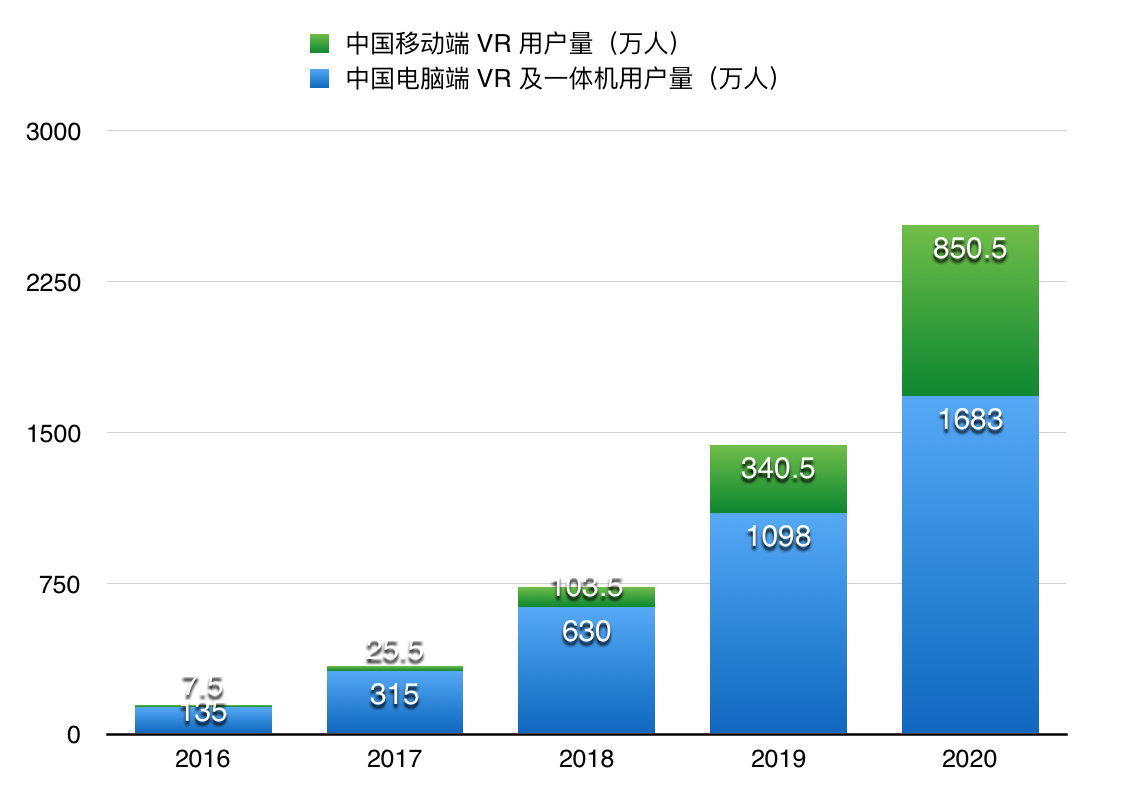
\includegraphics[width=.4\textwidth]{market}
\caption{2016-2020 年中国 VR 用户规模}
\label{fig:market}
\end{figure}

\section{全景漫游产业类别}
全景漫游产业按出发点可大体分为两类:
\begin{itemize}
	\item 以视频、游戏为主的虚拟内容提供商/平台商
	\item 涉及电商、教育、医疗、建筑等传统行业的行业融合应用服务商
\end{itemize}

短期而言,市场上比较活跃的是虚拟内容提供商,但长远而言,ToB 模式更利于产生更为健壮的全景漫游服务体系,对于高质内容的生产、分发和变现的模式也偏向于有传统大规模企业的行业服务商。

\section{全景漫游现有 APP 分析}
\subsection{Ascape}

Ascape 这款美国公司开发的应用于 2017 年发布,主攻虚拟旅游市场。你能够通过 360° 无缝的全景视频身临其境般地切身体验视频中呈现的著名景点或人文古迹,探索只有历经千难万险才能体会的绮丽风光。伴随着你的移动,场景中镜头也会随之改变整个画面的位置和显示的角度,见图\ref{fig:ascape1}。

\begin{figure}[htp]
\centering
\fbox{
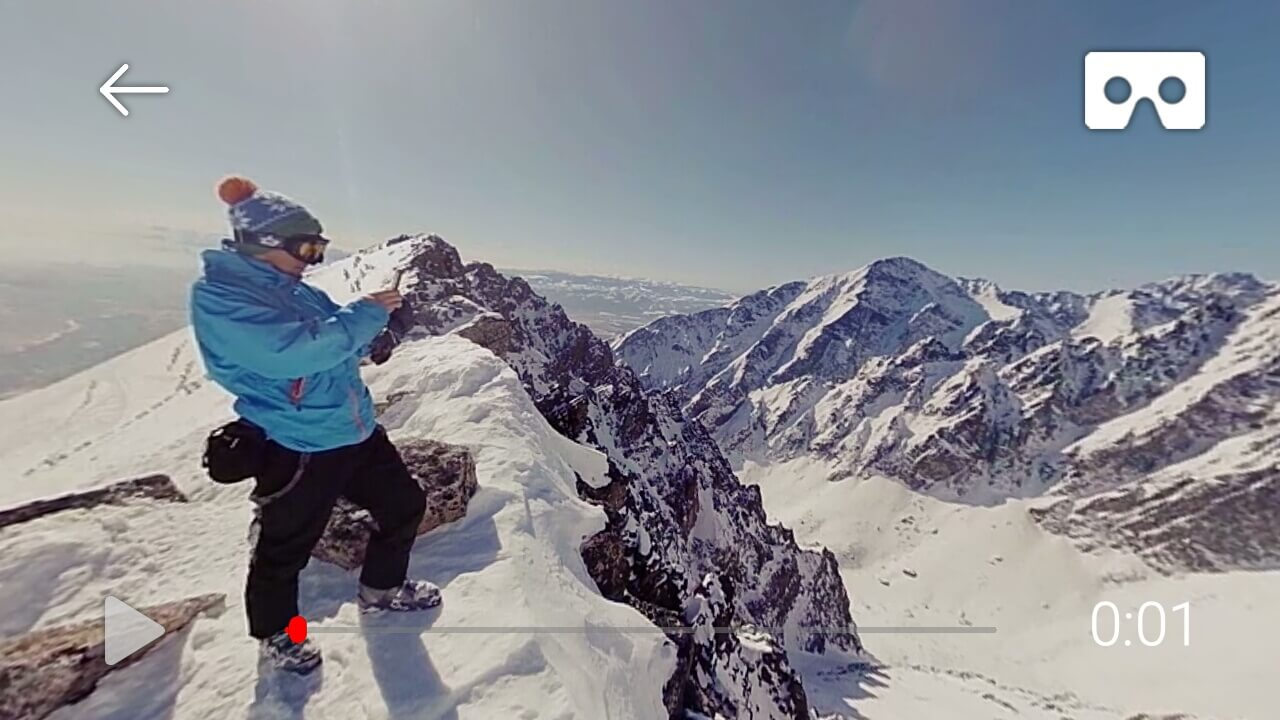
\includegraphics[width=.7\textwidth]{ascape2}
}
\caption{简洁的全景视频播放}
\label{fig:ascape1}
\end{figure}

同时,这款应用在移动应用传统界面上也继承了欧美一向以来的简约风格:“探索”页面采用卡片设计模式直观展示了新奇的场景;“发现”页面通过地图和名单两种模式展示了全球各地的场景选项;“我的旅行”也通过卡片模式展示了已下载的全景场景,见图\ref{fig:ascape2}。

\begin{figure}[htp]
\centering
\fbox{
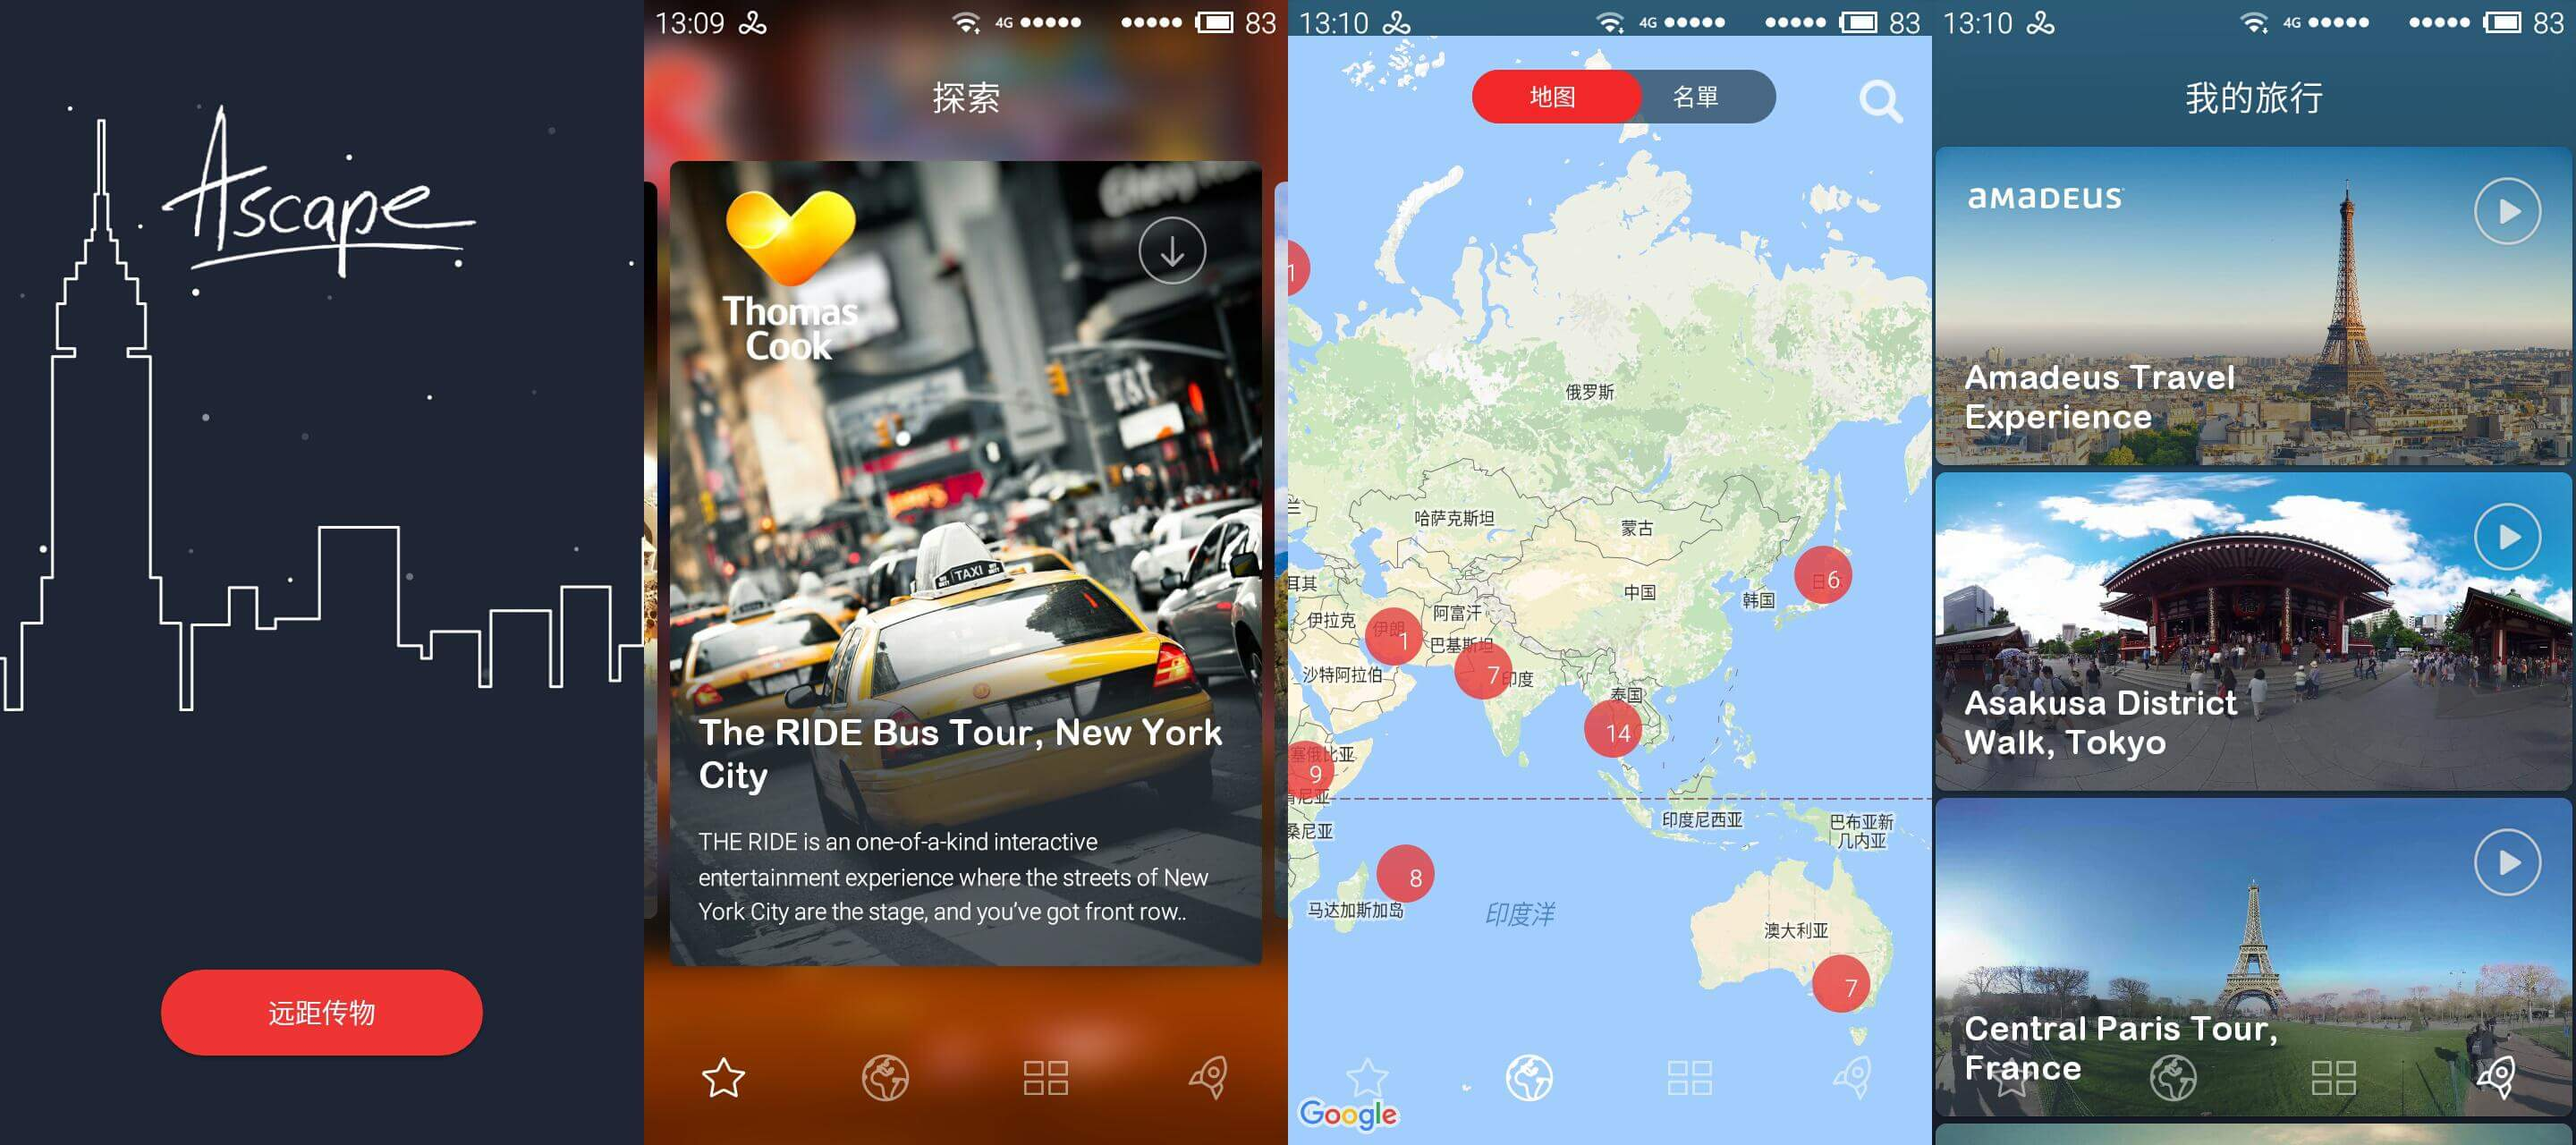
\includegraphics[width=.7\textwidth]{ascape1}
}
\caption{简洁的全景视频播放}
\label{fig:ascape2}
\end{figure}

\subsection{Fulldive}

Fulldive 这款美国公司开发的应用于 2016 年发布,是一个智能手机与虚拟场景连接的平台,进入应用后即进入了一个全景漫游的世界。场景内包含常用的网络视频、本地视频/图片、VR 相机、VR 浏览器等应用,同时支持从其内部市场下载更多基于其开发的虚拟现实应用,见图\ref{fig:fulldive1}。

\begin{figure}[htp]
\centering
\fbox{
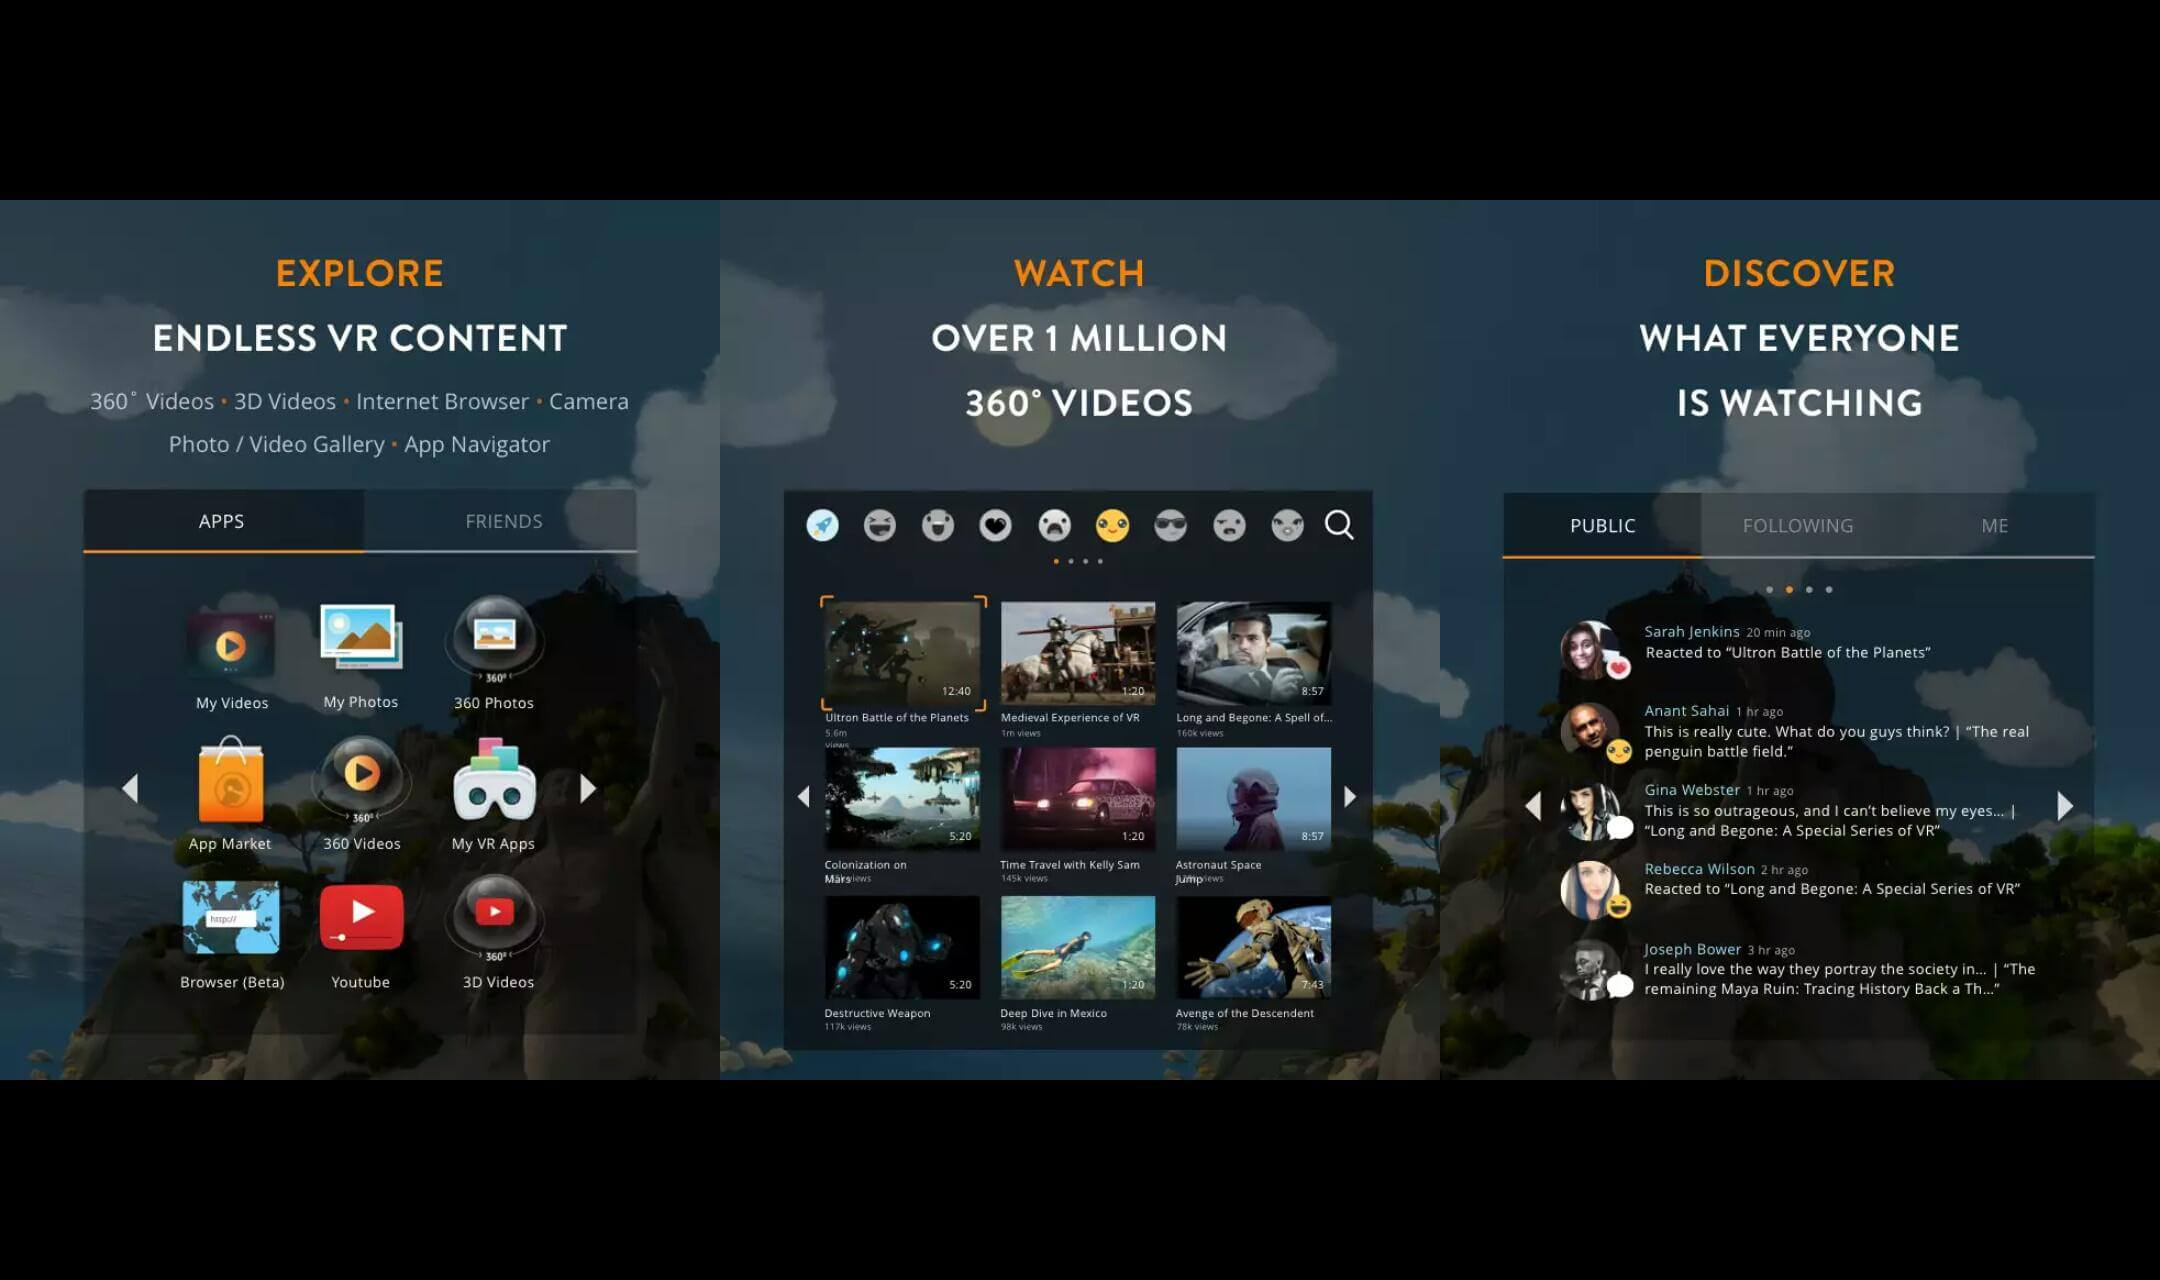
\includegraphics[width=.7\textwidth]{fulldive1}
}
\caption{Fulldive 内置的应用列表}
\label{fig:fulldive1}
\end{figure}

与 Ascape 不同之处在于 Fulldive 的操控完全是在虚拟全景中,所以在播放视频及操作选项时 Fulldive 有一些针对配戴虚拟现实眼镜者所特别提供的操作方式,见图\ref{fig:fulldive2}。例如,将视线聚焦在某个按钮上超过 3 秒后即视为按下了该按钮。这种交互形式借鉴了鼠标的双击或是触屏的长按这两种操作,同时兼顾到视线对齐对人操作的便捷性和可操作性,见图\ref{fig:fulldive3}。

\begin{figure}[htp]
\centering
\fbox{
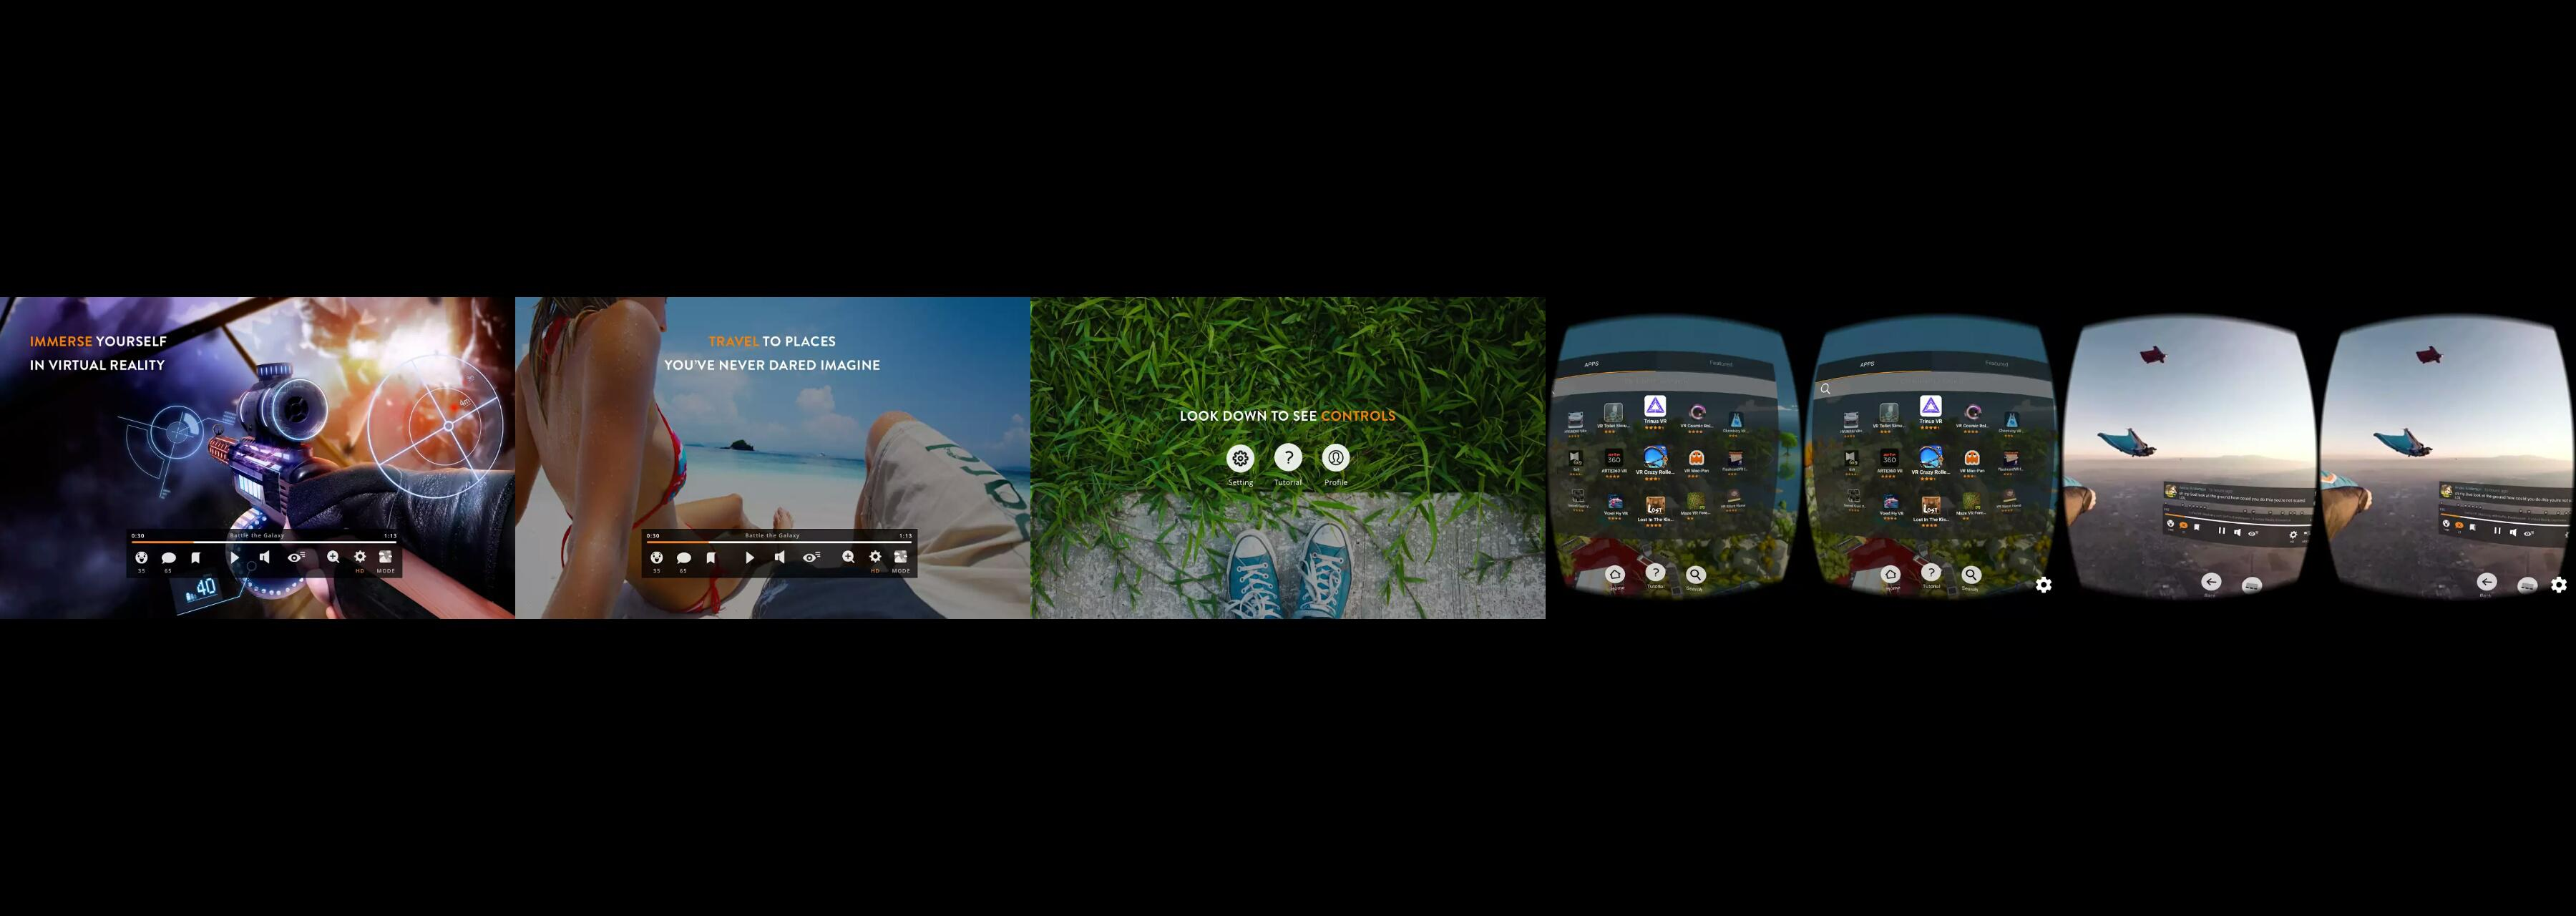
\includegraphics[width=.6\textwidth]{fulldive2}
}
\caption{Fulldive 特有操作形式}
\label{fig:fulldive2}
\end{figure}

\begin{figure}[htp]
\centering
\fbox{
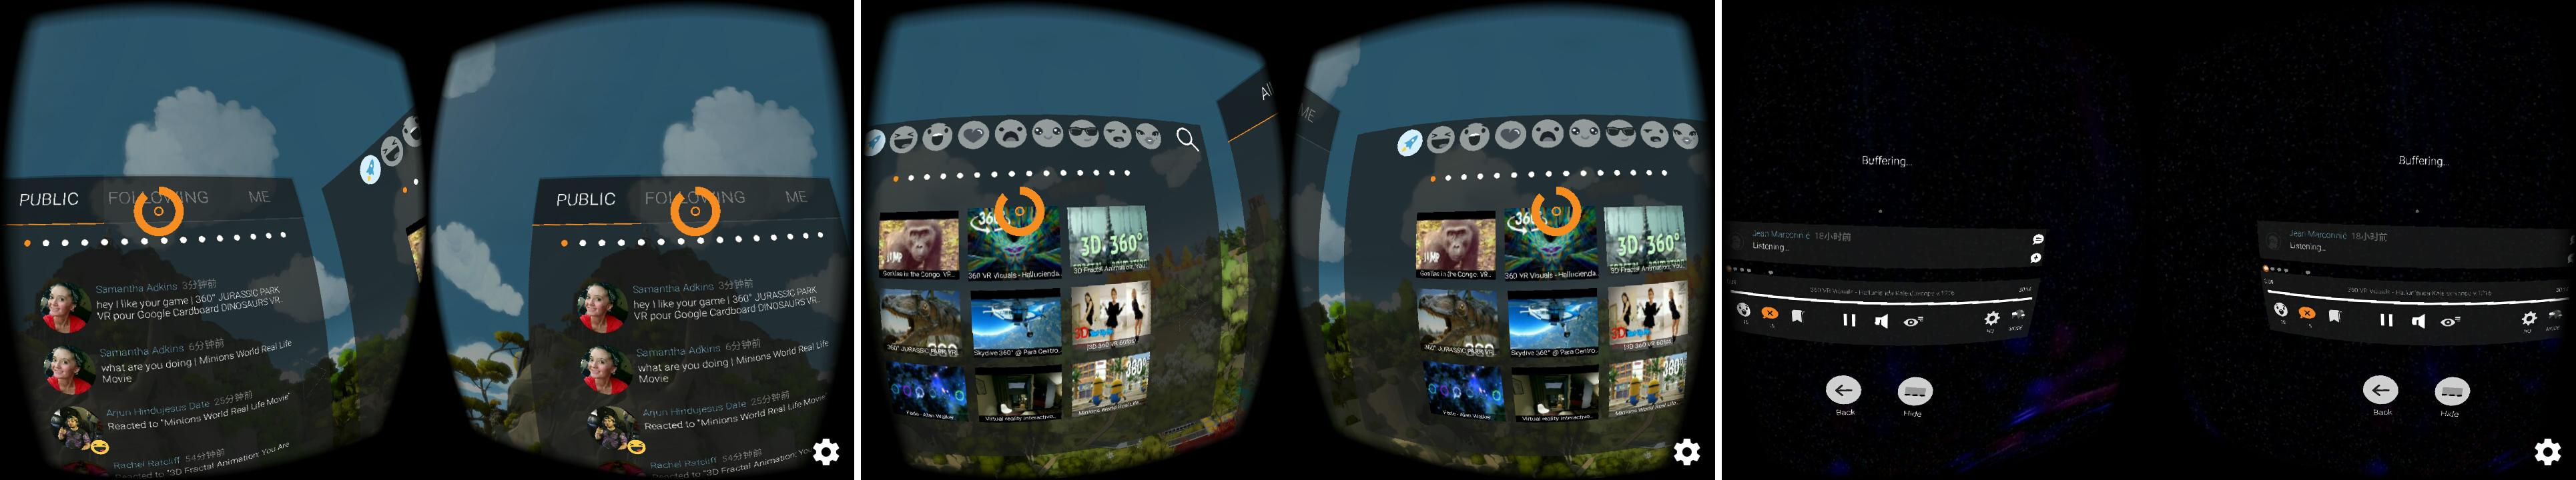
\includegraphics[width=.6\textwidth]{fulldive3}
}
\caption{Fulldive 视线停留模拟点击}
\label{fig:fulldive3}
\end{figure}

当然,这种模拟点击的操作只适用于”确认/取消“这种布尔判断的操作,用户需要输入大段的文字时则需有更高效的方式。Fulldive 结合了已日益成熟的语音识别技术,图\ref{fig:fulldive4}为实际操作 Fulldive 搜索功能并口述”中国地质大学“后的操作截屏。

\begin{figure}[htp]
\centering
\fbox{
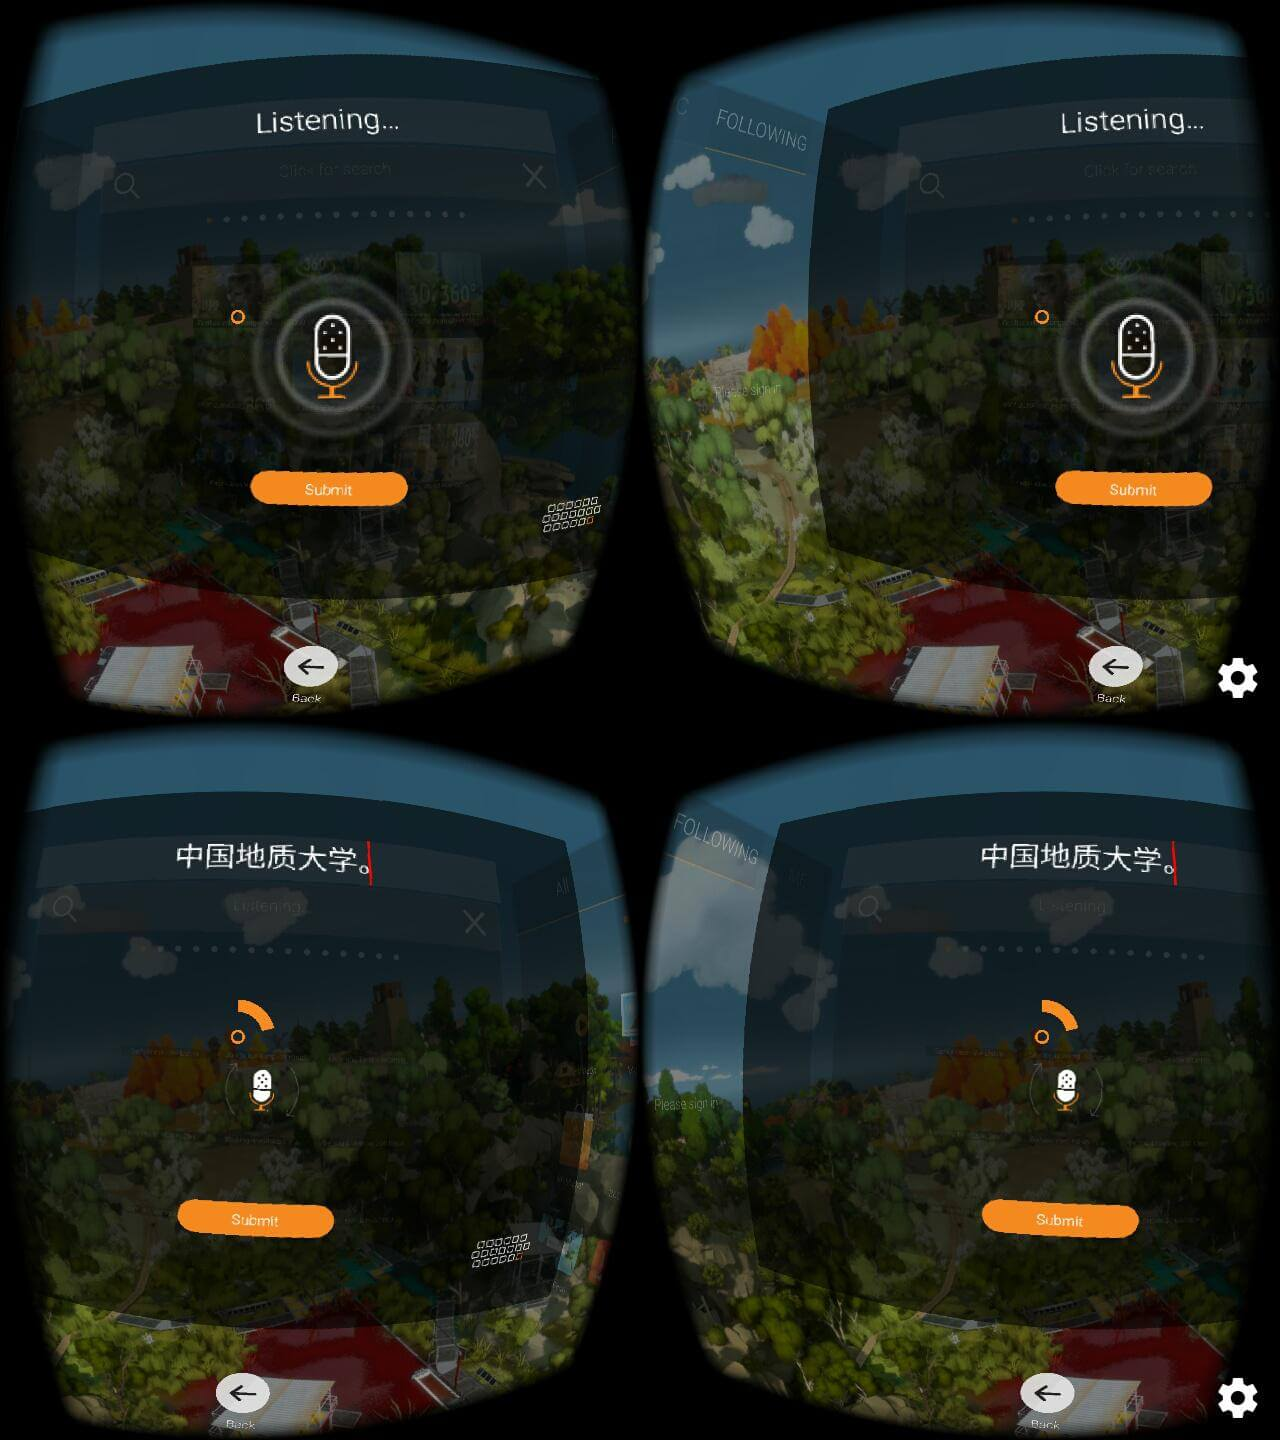
\includegraphics[width=.5\textwidth]{fulldive4}
}
\caption{Fulldive 语音识别}
\label{fig:fulldive4}
\end{figure}

\subsection{VR X-Racer}

VR X-Racer 是一款越南公司于 2016 年开发的简单的 VR 操控类飞行游戏,其操作方式为晃动设备(如 VR 眼镜或手机)来控制屏幕上的飞机躲避障碍物,见图\ref{fig:x-racer}。这是全景漫游技术在游戏上最直接的体现:几乎没有多余的操作,在游戏中飞机撞到障碍物坠毁后无操作若干秒即自动重新游戏。但其最大的缺陷是无法长时间使用,不断晃动的全景屏幕容易使人产生眩晕、恶心等不良反应。
全景漫游与 3D 影片的体验是完全不同的,全景漫游将用户完全包裹在视频所构建的封闭环境中,而 3D 眼镜只是对屏幕这种有限区域进行了折射。两者的区别在于 3D 影片由于有周围环境作为铺垫不易使人完全沉浸其中,全景漫游则是在很短的时间内(20-30 秒)就使人沉浸在虚拟世界中,直至摘掉全景设备重新适应周围环境。

\begin{figure}[htp]
\centering
\fbox{
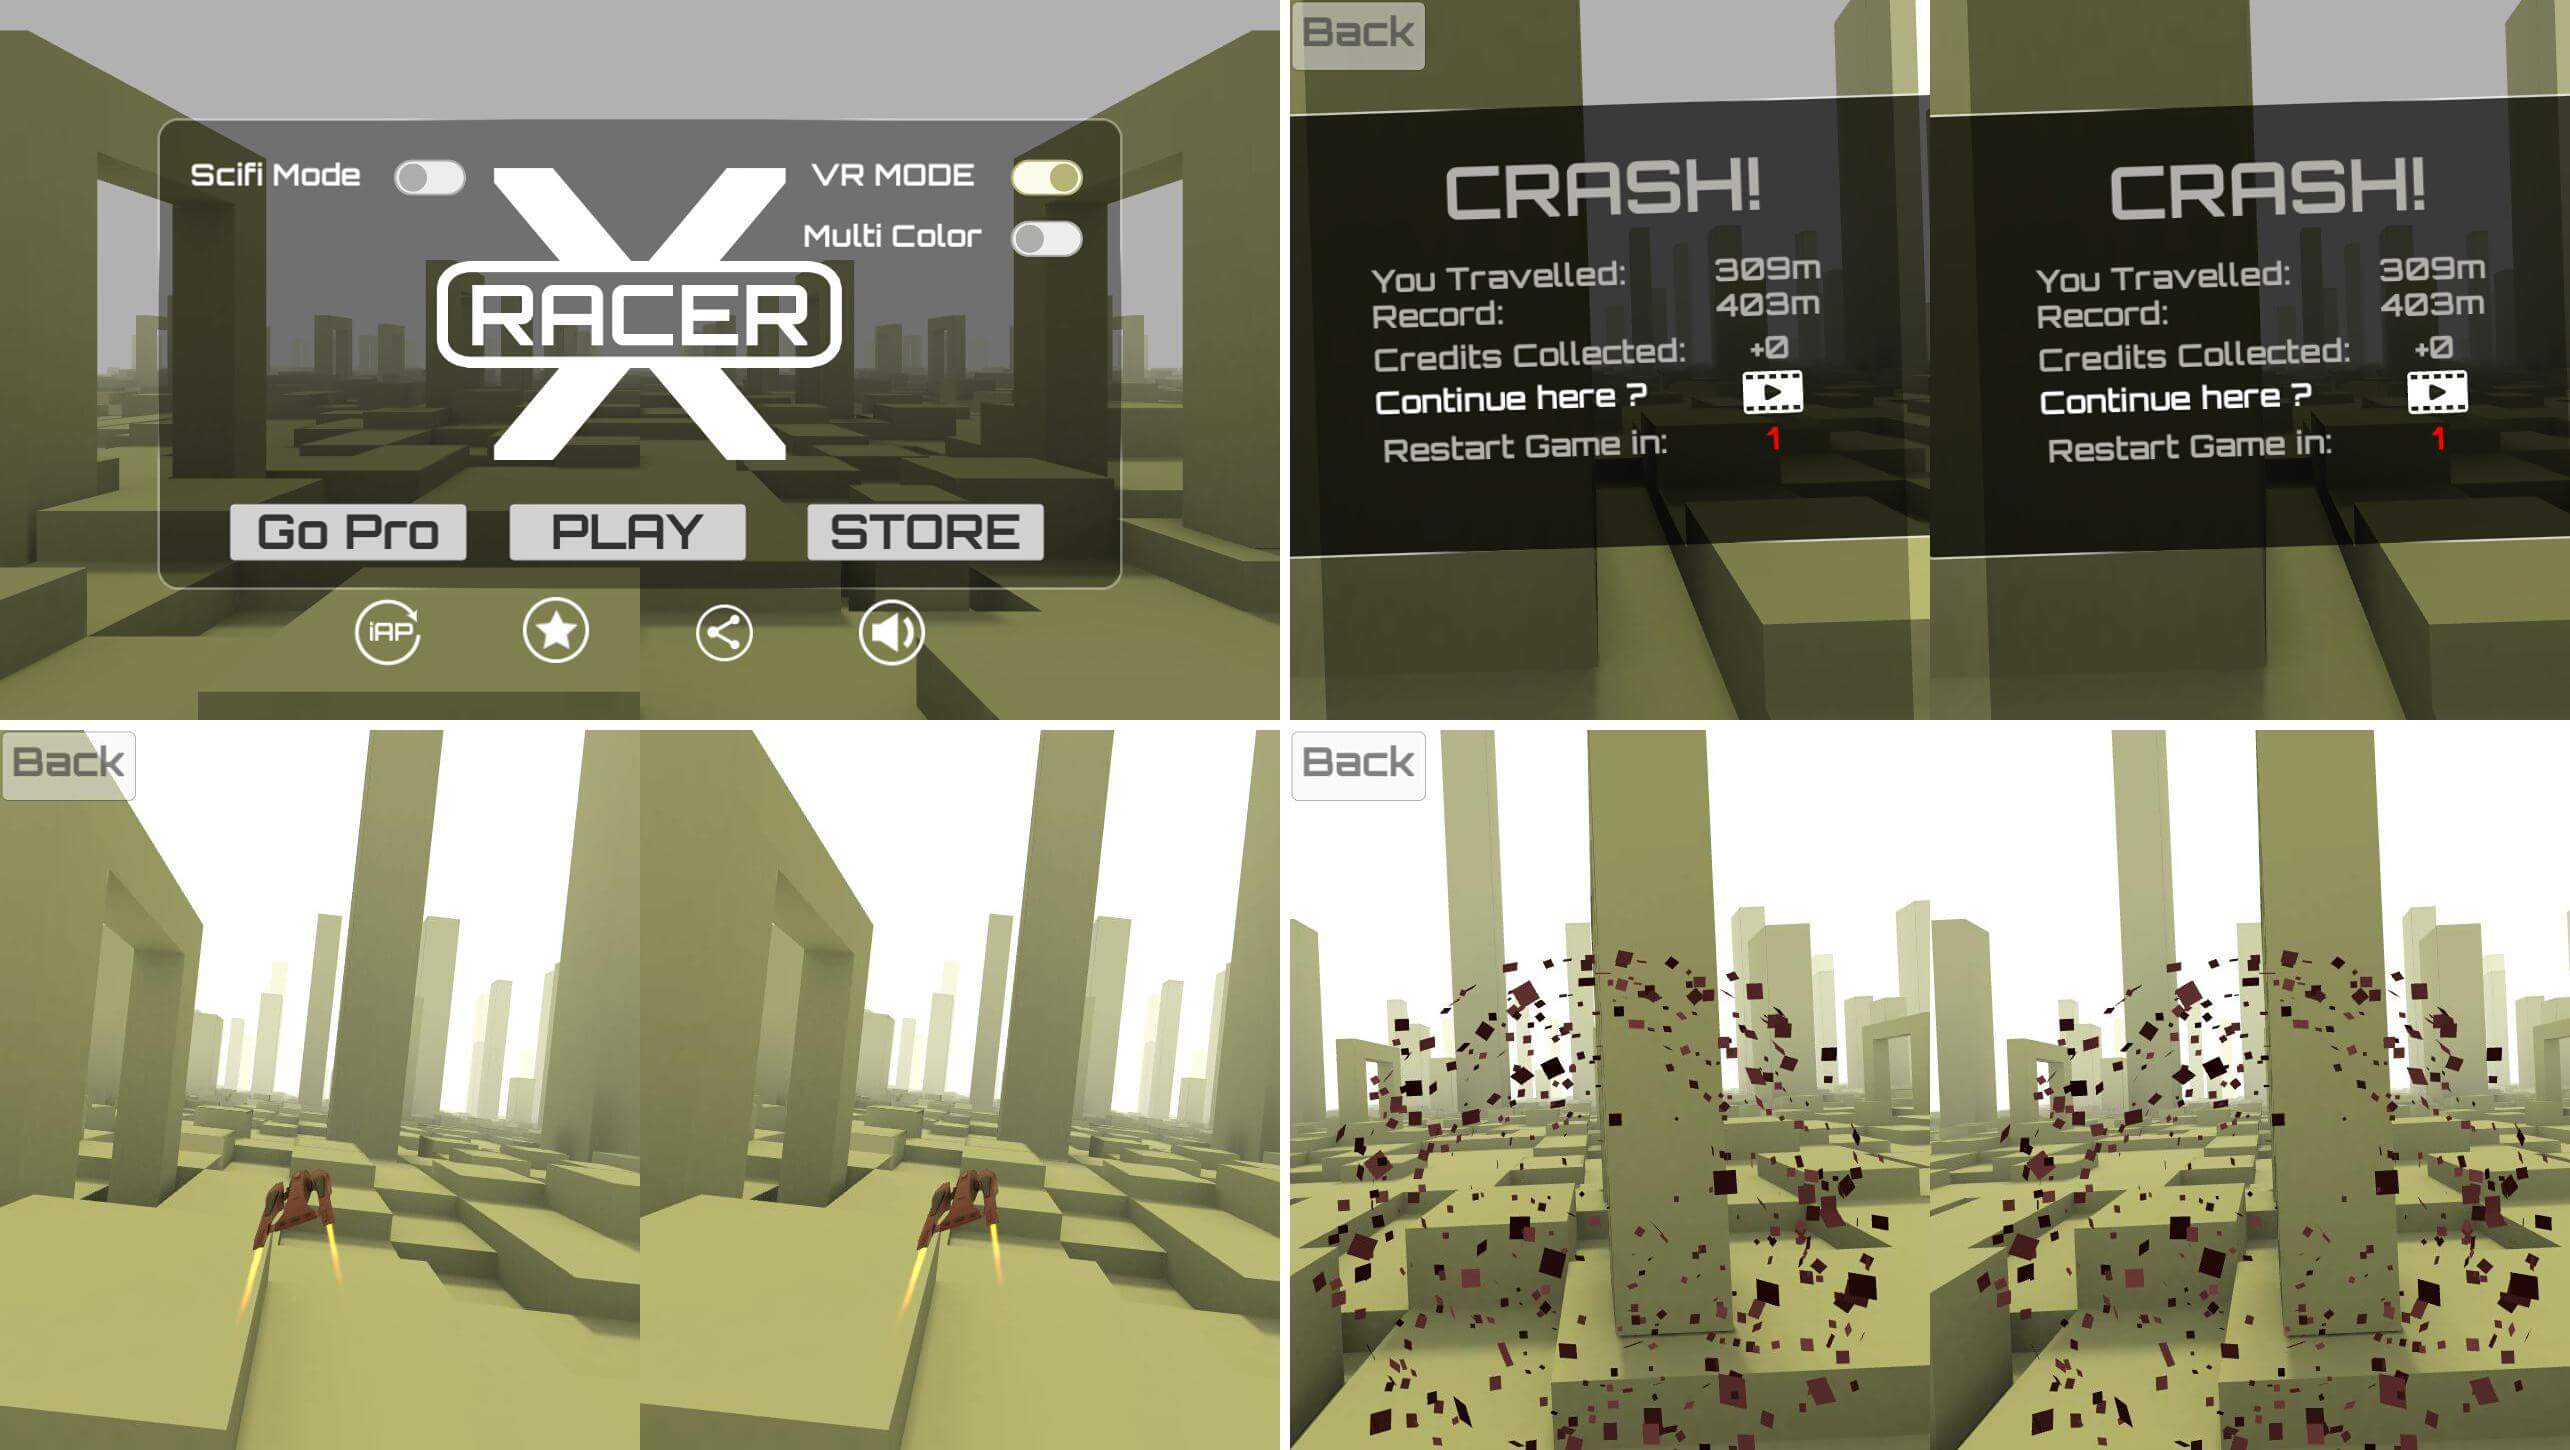
\includegraphics[width=.5\textwidth]{x-racer}
}
\caption{X-racer 游戏截图}
\label{fig:x-racer}
\end{figure}

\subsection{暴风魔镜 VR}

暴风影音是国内在全景漫游生态领域探索前沿的产品之一,最早产品发布于 2014 年,其高端产品售价可达数千元,甚至与国外高端虚拟现实设备如 Oculus 和 GearVR 等价格相齐。与其硬件设备配套的则是一款叫做“暴风魔镜 VR”的手机移动应用。

国内移动应用的发展方向一直是“大而全”,这款应用也不例外。暴风魔镜 VR 力图包括网络/本地视频、影音播放与 VR 移动应用等多种应用,形成自己的 VR 平台体系。该应用不但支持普通的移动应用界面操作模式并且同样支持全景漫游的虚拟现实体验模式。

在交互形式上与上文所列举的 Fulldive 类似,均为视线聚焦停留数秒视为确认,但缺少了语音识别输入大段文字的功能(在页面模式下支持手机输入法输入),如图\ref{fig:storm}。总体使用可满足基本的全景漫游体验,但识别速度较慢或误识别是比较严重的问题。

值得注意的一点是,暴风魔镜 VR 移动应用内场景下方有一个“归位”图标,触发后将会调整屏幕主视域至正对当前屏幕的位置,可类比于传统移动应用的“回到顶部”功能。这个功能很方便地起到了定位自身的作用,让用户不必盲目转动来寻找起始时正对着的界面。


\begin{figure}[htp]
\centering
\fbox{
  
\includegraphics[width=.22\textwidth]{storm1}
}
\fbox{
  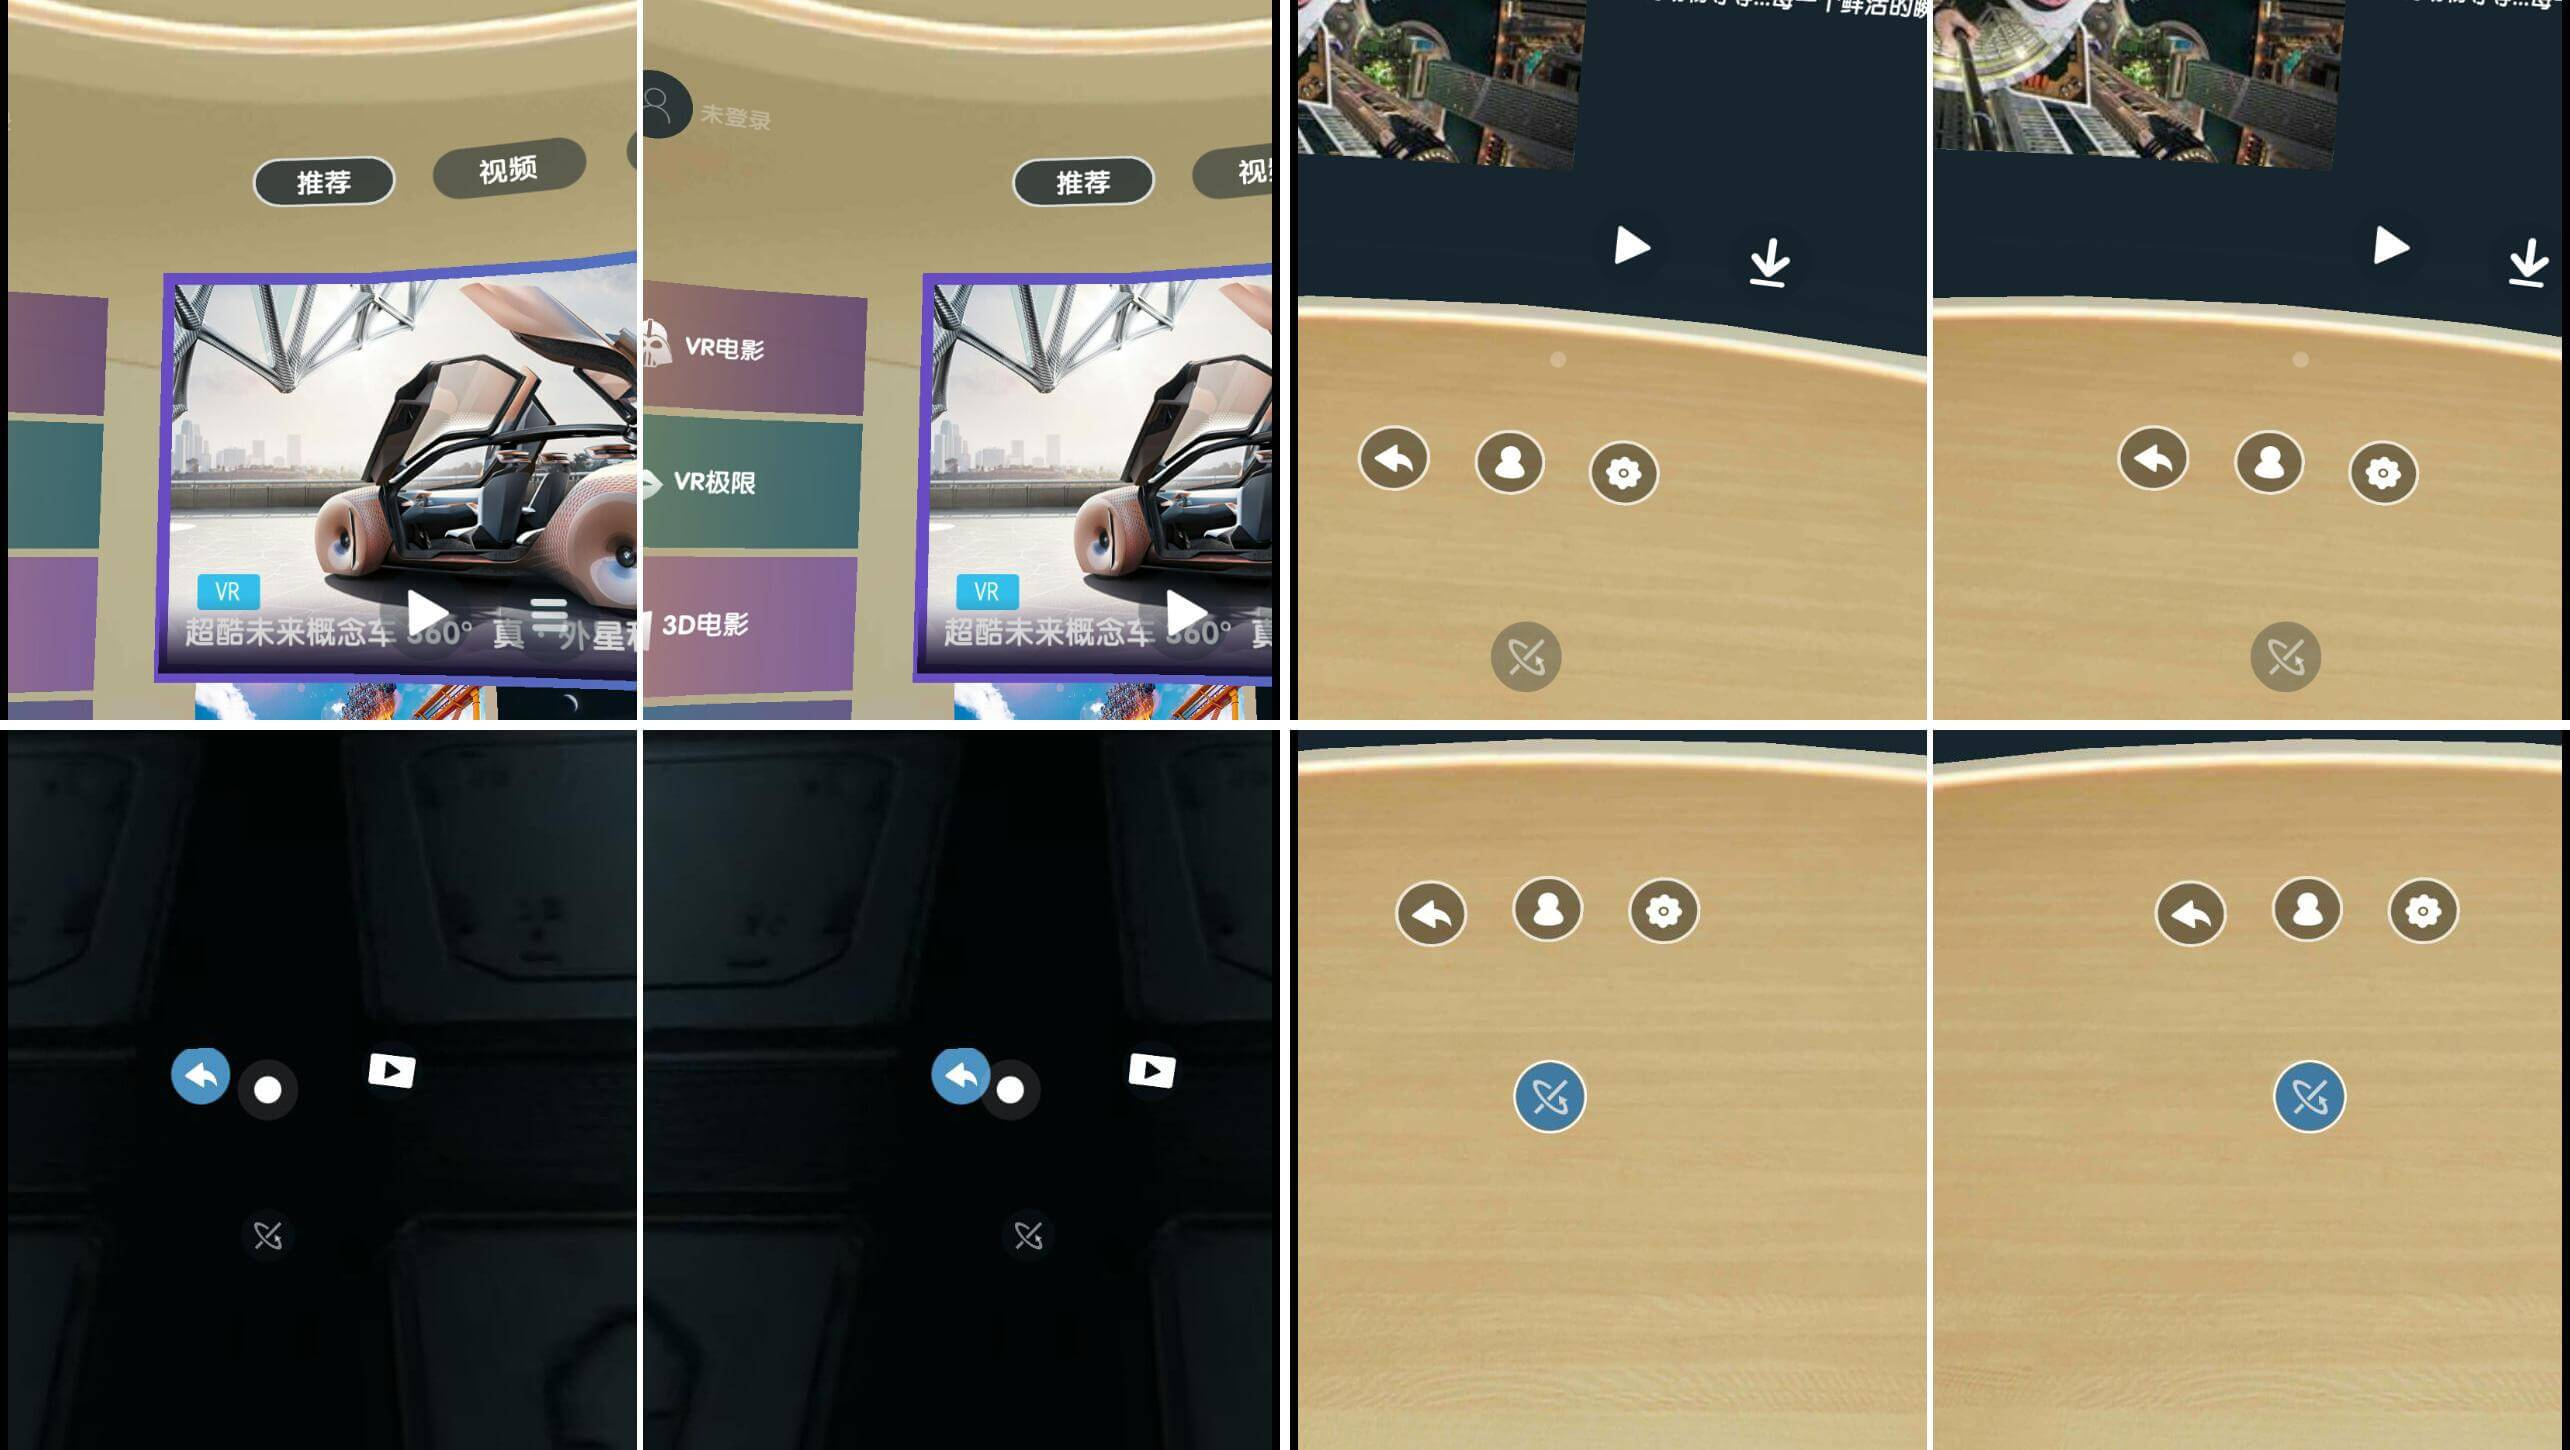
\includegraphics[width=.68\textwidth]{storm2}
}
\caption{暴风魔镜 VR 操作方式}
\label{fig:storm}
\end{figure}

\subsection{国内外移动应用总结}
国外应用较多为单一功能并凸显自身用户体验特色,而国内应用多期望建成平台式产品力图获得更大的市场份额。究其原因,国外此类开发团队小而精,立足于开发特定使用情景和目的的产品,而国内应用常常依附于配套开发的硬件设备,整体呈闭源趋势,故应用局限性较大。国外应用功能较为精简,国内应用则力图提供尽可能多的交互操作形式,但同样在交互层面难以摆脱移动设备平面屏幕所框定的范围。


\section{全景漫游行业现状总结}

全景漫游正处在行业发展的成长期,相关技术发展迅速,但同质化较为严重。众多厂商基于经济利益考量注重硬件设备的研发和更新换代,但软件质量与硬件质量仍有一定的差距,主要体现软件交互设计的质量上。

在全景漫游的交互设计上,国内外 APP 均有较多针对与不同与传统人机界面交互的创新点,例如前文列举的“视线停留数秒确定”、“语音识别”和“底部 Docker 栏”等。但交互可操作性相比于传统人机界面还有一定的差距,例如无法很快定位到所需内容、运动过程中不易操控等问题。同时,在全景漫游的现有设计中,仍旧无法脱离面向传统人机界面的设计语境,在考虑保留用户习惯的同时难以创新出更为独特的交互模式,可以说是全景漫游交互设计亟待研究的难点。

全景漫游的行业发展离不开全景漫游的软硬件及生态环境的良好结合,只有如此才能留存有效用户并产生价值,故行业目前的重点就是在软硬件上均体现出应有的价值提升。其中,软件方面可在全景漫游领域的交互方向结合相关理论作出新的设计以改善用户体验。

\chapter{全景漫游与人的关系}

\section{全景漫游的生理行为特性}
实现全景漫游与传统人机界面最大的区别在于全景漫游时的设备(包括 VR 眼镜或专用眼罩)距离人眼只有 2~3 公分距离,设备整体对人眼呈包裹状态。使用者仅可通过听觉和其他一些不够灵敏的感觉来感受外界环境,使用环境的舒适性就变得非常重要。

全景漫游与人体关联的感觉和生理运动大致有:视觉、听觉、肢体运动等。如图\ref{fig:human_sence}。

\begin{figure}[htp]
\centering
\fbox{
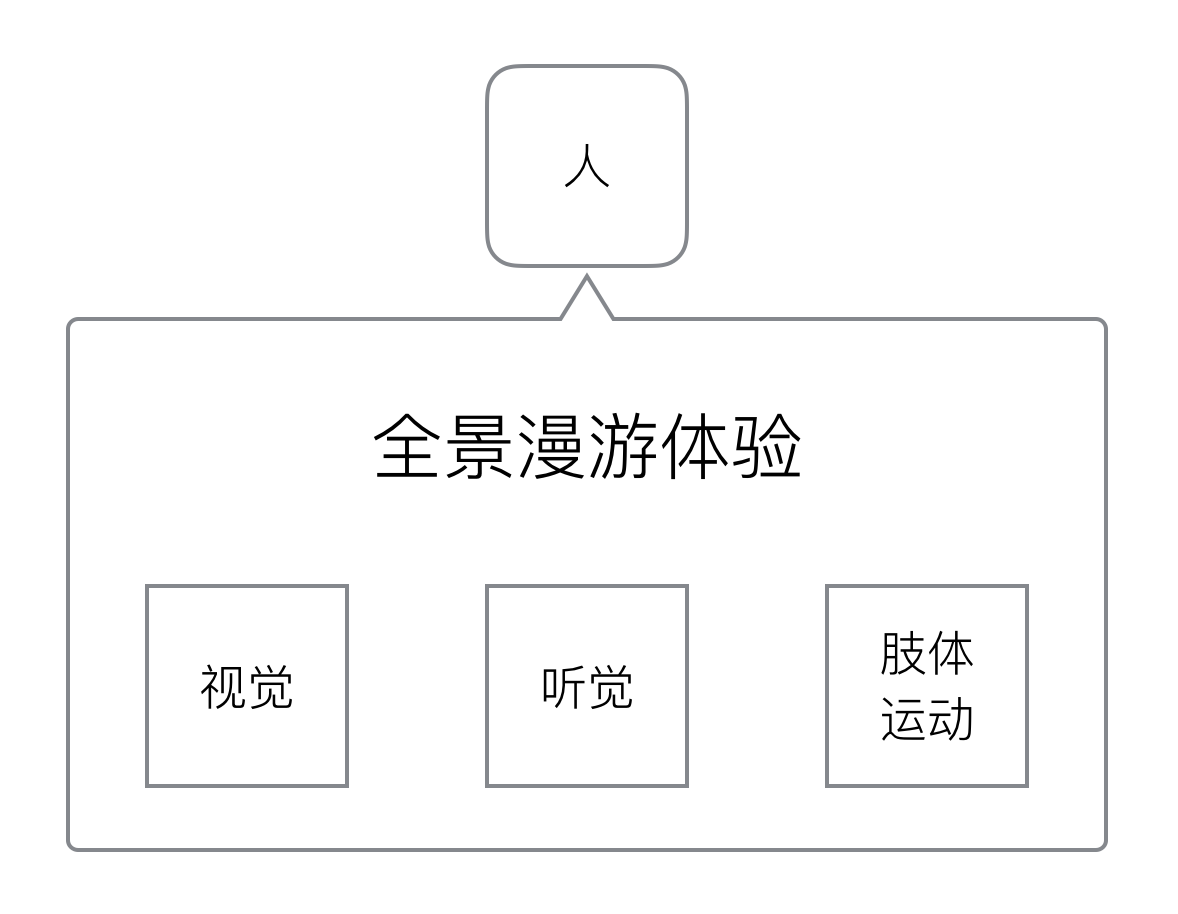
\includegraphics[width=.5\textwidth]{human_sence}
}
\caption{全景漫游与人体知觉}
\label{fig:human_sence}
\end{figure}

\subsection{全景漫游与视觉特征}
全景漫游对人体最大的刺激来源即是视觉刺激,其特征为距离眼睛距离近,色彩、明暗、动作变化等刺激较一般显示屏幕会更为剧烈。

\subsubsection{视角与视野}

人的视角是确定被看物尺寸范围的两端点光线射入眼球的相交角度。视角的大小与观察距离及被看物体上两端点的直线距离有关,其计算公式\ref{eq:angle}如下:
\begin{equation}
\alpha=2\arctan{\frac{D}{2L}}
\label{eq:angle}
\end{equation}

其中,$\alpha$ 为视角,用 $(^{\prime})$ 表示,即$(1/60)^{\circ}$单位;D 为被看物体上两端点的直线距离;L 为眼睛到被看物体的距离。
如果设眼球距镜片距离为 1.5cm,而镜片上一物体显示高度为 2cm,则带入公式可得\ref{eq:data}

\begin{equation}
\alpha=2\arctan{\frac{2cm}{2*1.5cm}}\approx 67.38 ^{\circ} = 2 \times 38.69^{\circ}
\label{eq:data}
\end{equation}

即上下视角各约为 $38.69^{\circ}$,查阅数据可知人在垂直平面的视野最大视区为视平线以上 $50^{\circ}$ 和视平线以下 $70^{\circ}$,颜色辨别界限为视平线以上 $30^{\circ}$,视平线以下 $40^{\circ}$。

由上述计算可知,在使用全景漫游设备观看场景时,假设高为 2cm 的显示物体在人视野中上部已超出颜色辨别界限,下部也已接近颜色辨别界限。物体上部比下部更接近垂直平面内的视野极限,如图\ref{fig:angle}。由此可知,全景漫游场景设计中应将主要元素置于屏幕中央,次要元素尽可能置于屏幕下方以便识别操作。同时,色彩丰富且饱和度高的元素也应置于视野中部,而一些操作类的元素则不应用过于丰富饱和的色彩缀饰,以免让使用者应难以分辨色彩而操作出错。

\begin{figure}[htp]
\centering
\fbox{
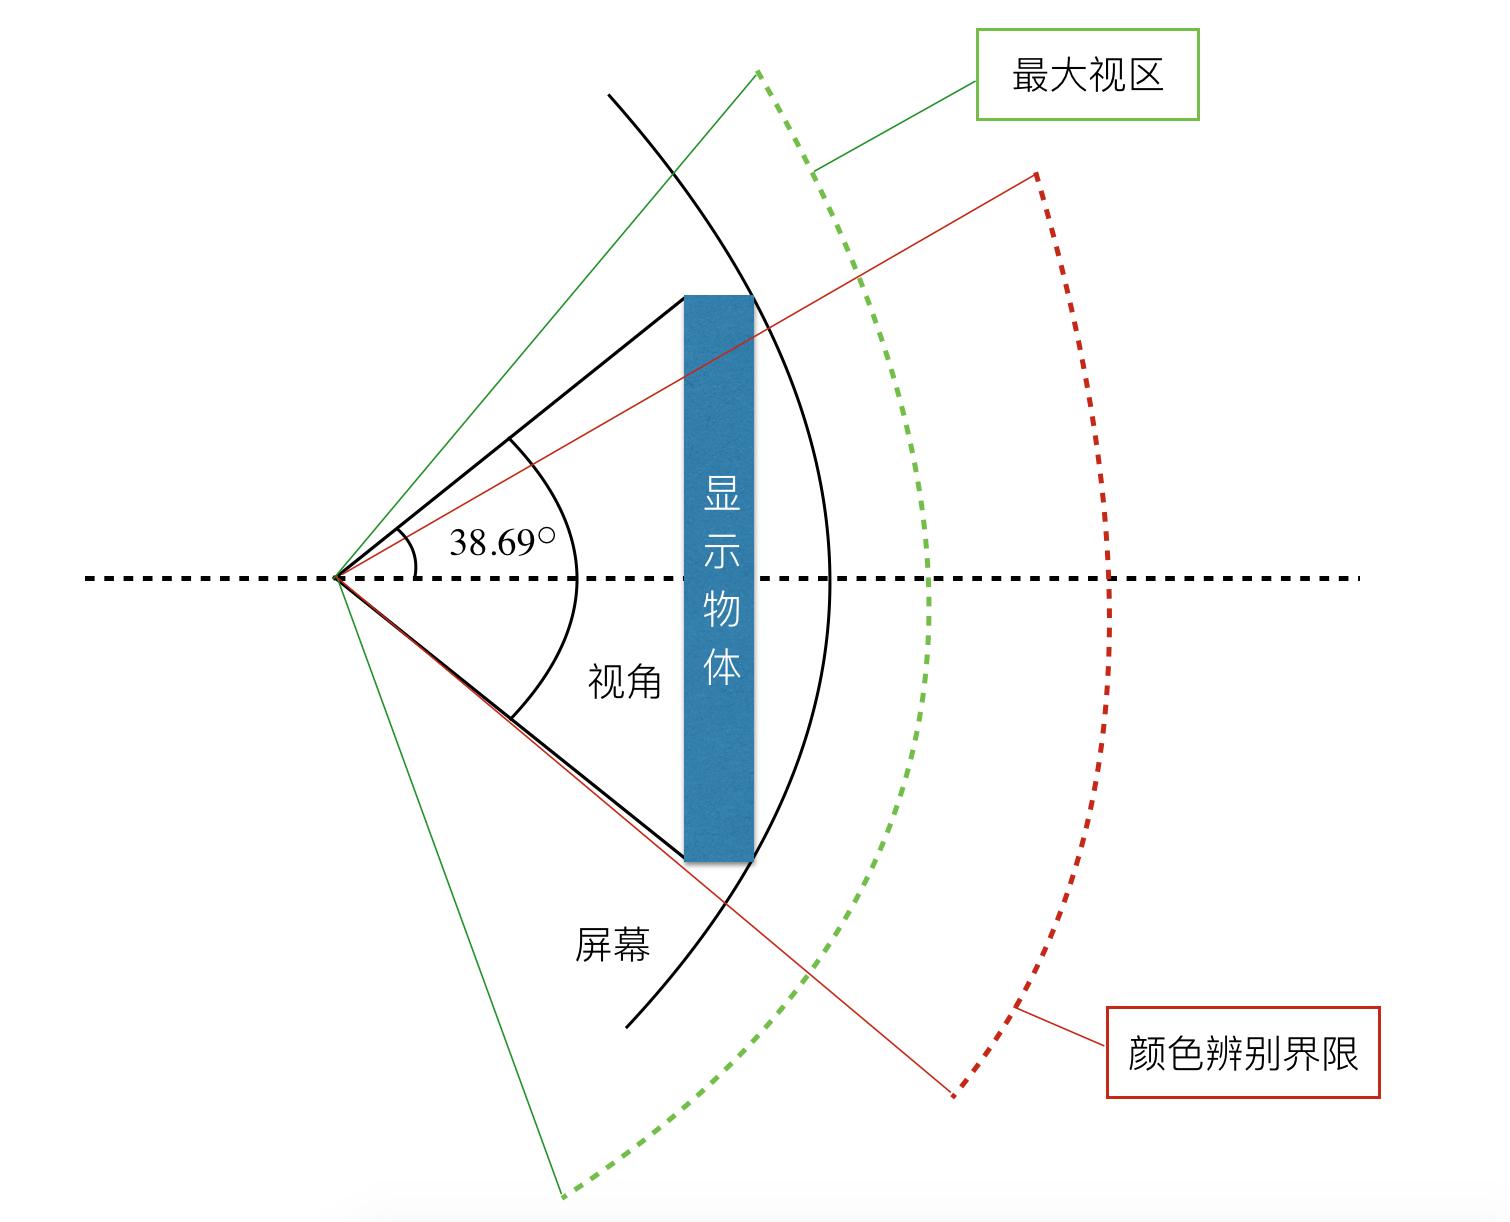
\includegraphics[width=.7\textwidth]{angle}
}
\caption{全景漫游中视野的角度关系}
\label{fig:angle}
\end{figure}

\subsubsection{视觉适应}

配戴全景漫游设备进行观察时,屏幕距眼球距离不足 2cm,属于视距过近状态,应当避免长时间操作,否则易引起眼睛疲劳。同时由于屏幕与眼球距离过近,屏幕亮暗对眼球刺激比通常工作环境更为强烈。当屏幕上场景切换间明暗变化过快时,人眼需要一定的适应时间才能正常分辨,但由于全景漫游设备等封闭性,无法较轻易地脱离这种明暗急剧变化的环境,则眼睛无法得到充足有效的适应时间,则很容易产生视觉疲劳,影响视觉能力。

\subsection{全景漫游与听觉特征}

全景漫游的视觉是主要人体感觉,但听觉是仅此于视觉的重要感觉,尤其是在视觉被全景场景完全包裹住的情况下。

现有全景漫游设备有的自带耳机设备,也有的需要自行配备耳机。但长远来看,配备耳机可能是必然的选择。因为人耳具有“方向敏感度”(或称“双耳效应”),即:声波在进入鼓膜时,受人体的反射、折射和衍射而扭曲变形,大脑能根据经验判断出声源的方位和距离。而前文所说的“耳听八方”即说的是这种能够重建场景音效的能力。

\subsubsection{双耳效应}
为了“制造”出能够“蒙骗”大脑使其误以为使用者身处虚拟场景中的体验,大致方向是重建出空间任意一点至双耳处的滤波器函数。我们不必去关心空间中某一点的声波是如何传播到人耳中的,只需要将该点声波信号经过滤波器便可以得到它在人耳处的声波信号,如图\ref{fig:hrtf}。而这个信号是可逆的,即被人耳捕捉到之后便由大脑还原成相应位置的“声信号”,从而达到“欺骗”大脑的目的。这个领域的研究对象叫做 HRTF(Head Related Transfer Function):头相关变换函数,是一种音效定位算法。但每个人的听觉能力都是不同的,所以 HRTF 对人类整体并没有通解,而只有对于人类个体经过反复实验测试后的特解。

\begin{figure}[htp]
\centering
\fbox{
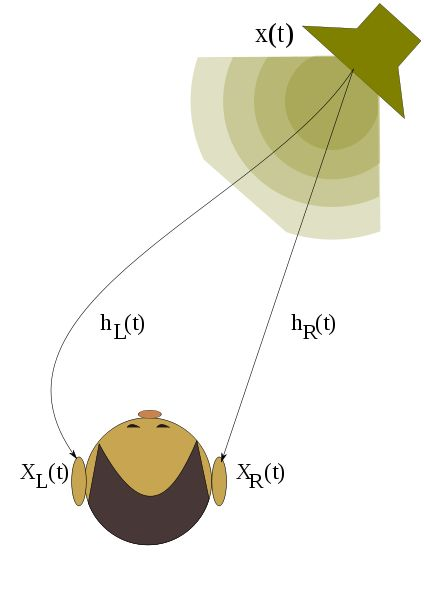
\includegraphics[width=.4\textwidth]{hrtf}
}
\caption{头相关变换函数 HRTF}
\label{fig:hrtf}
\end{figure}

国内外已有厂商根据相关理论设计并制作出了 VR 耳机,可配合 VR 眼镜使用,也可独立使用,它会追踪使用者的姿态、位置变化等,进而计算并还原出模拟三维场景内的声音分布,让使用者仿佛置于真实的场景之中。

\subsubsection{视觉的「补充」}
虽然声音不是可视化领域的研究重点,但良好的听觉体验的确有利于信息渠道的建立。视觉与听觉互为补充、相互作用、最终是人的知觉更为敏锐而准确。可以设想以下场景:「用户配戴全景漫游头盔进行一场探险类的游戏,用户扮演的主人公正在探索未知的世界,正当主人公小心翼翼地穿过一片沼泽时,后方突然传来了一声尖叫…… 」如图\ref{fig:audio-source}看不见的事物通过音效来表现,可以提升场景所渲染出的气氛效果。听觉与视觉不同,不受方向影响,能够用来表现一些视觉上无法做到的特殊效果。

\begin{figure}[htp]
\centering
\fbox{
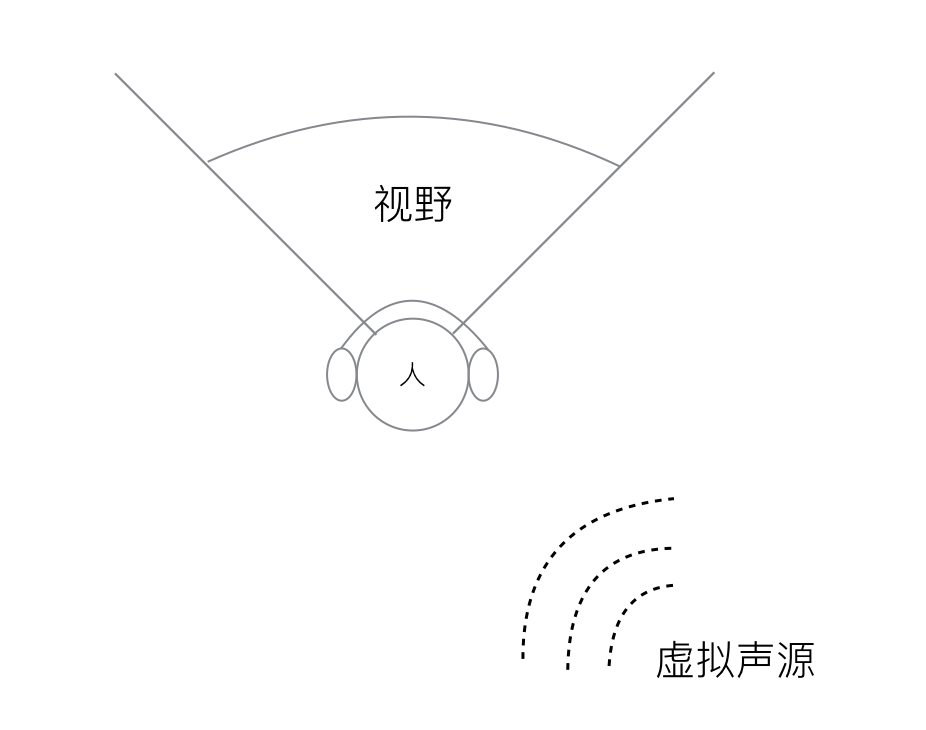
\includegraphics[width=.5\textwidth]{audio-source}
}
\caption{用音效来表现「看不见」的事物}
\label{fig:audio-source}
\end{figure}

\section{全景漫游与肢体动作}

全景漫游,其一是“全景”,其二则是“漫游”。漫游,意为随意游玩、漫无目的地行走。全景漫游的体验重在参与感的营造,用户不仅能够“身临其境”般地体验全景场景,更可以亲身参与其中,与场景中的虚拟事物进行互动。

\subsection{平衡感}
众所周知的是,人之所以可以站立行走、骑行脚踏车或进行高空作业依赖的是人与生俱来并在后天不断磨合的平衡感。平衡感由内耳的淋巴液控制,同视觉相互配合,使人能安全地四处走动。而在全景漫游过程中,人的视觉几乎全部集中在眼前的屏幕上,即很难看到外界真实的场景,故视觉此时便难以匹配内耳中内淋巴液流动引起的细胞兴奋,对人来说就是平衡感的缺失。失去平衡感会使人晕眩,严重时会使人倾倒,有造成意外伤害的可能,故在进行全景漫游时应尽可能减少乃至避免对平衡感造成的影响。

维持平衡感有两种方式,一种是降低运动的速率(即减小在全景漫游中需要运动的强度)视为主动维持平衡感,另一种是通过某些手段来减少视觉或其他感觉中平衡感的减少,即运动补偿,可视为被动维持平衡感。

现有全景漫游设备部分带有陀螺仪、部分利用手机内置陀螺仪用以感应方位信息,可做运动补偿以模拟人在环境中的运动,但人的眼球可以根据平衡来进行前庭—眼动反射 ( vestibulo-ocular reflex)控制眼球作补偿性运动,使之匹配头部的转向,以求维持人视野的稳定。这套机制在不戴全景漫游设备时可以正常运作,但在配戴了全景漫游设备后因眼镜视野与外界隔离,故设备与外界的运动匹配度就变得格外关键。

现有普通手机所内置的是微机电陀螺仪(MEMS),是利用物理学的科里奥利力,在内部产生微小的电容变化,通过测量电容,计算出角速度,从而判断物体转向和速度,这种芯片价格低廉,体积小巧,但缺点是因其电磁特性易受环境干扰,而且精度即使能够满足一般手机应用(如转屏、翻转等)但在更为精细的全景漫游的方位感应上还是显得力不从心。屏幕显示画面本身就有约 1/60s 即 16ms 左右的刷新时差,再加上陀螺仪反馈信息与实时状态也有偏差,两者累积后在使用者运动时画面很难及时更新至准确的位置上,容易造成失去平衡的感觉。甚至在人停止运动后,全景漫游设备错误地输出带有运动补偿的画面以致人眼误以为人体还在做运动,造成认知上的偏差,导致非运动状态下的感官刺激,这种刺激往往对使用者造成较长时间的影响,延续到使用完全景设备后的数分钟乃至若干小时后。

全景漫游技术的发展在维持人体平衡感方面尚有很大的发展空间,现有高端全景漫游设备即使是支持全方向漫游的平台也只允许使用者慢步使用,而运动补偿机制仍沿用着手机等终端的设计(大多数全景漫游设备并没有自己的陀螺仪,而是直接调取了与其连接的手机的重力感应接口)在需要高精度分辨的场合表现就达不到使用要求了。

\subsection{关节运动}

全景漫游人体主要运动可分解为躯干的平面运动和头部的转动,这两方面配合眼球的转动就构成了全景漫游中人个体在场景中的位移和转向,如图\ref{fig:act}。

\begin{figure}[htp]
\centering
\fbox{
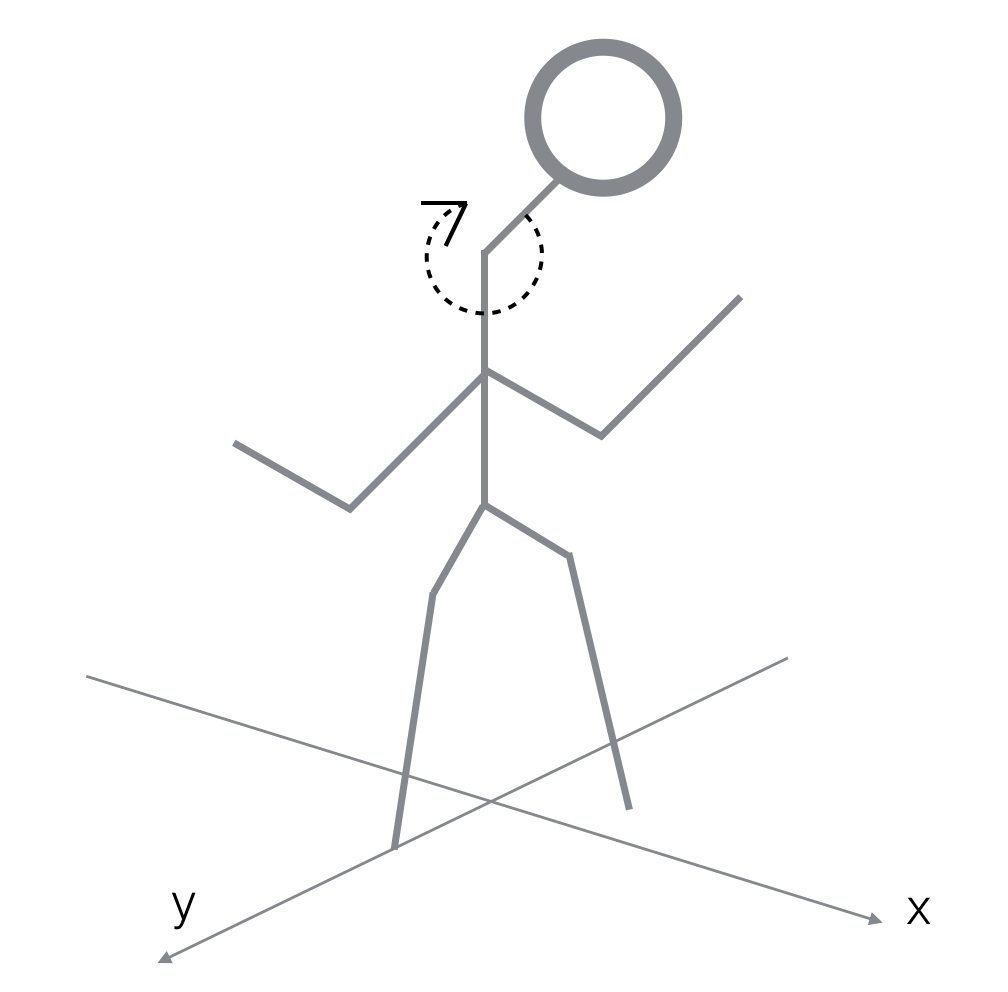
\includegraphics[width=.5\textwidth]{act}
}
\caption{躯干的平面运动与头部的转动}
\label{fig:act}
\end{figure}

但躯干的平面运动一般受场地的制约,并不是绝对的自由行进,而且由于人在看不到外界环境时处于一种对外界警惕的状态,实现行走不是全景漫游最优的运动方式。头部的转动则是一种比较好的选择,首先它的运动幅度较小,易于控制,其次头部转动也是人本能的反应,符合人对场景活动的预期。

人头部转动的形式有以下几种:低头与仰头、左歪与右歪、左转与右转。低头仰头的最大范围为 75°,另两种形式都为 110°,但低头舒适范围为 25°,仰头舒适范围为 12°。由此可得,全景漫游所用观看形式仍应以正面为主,辅以左右延展开的场景以供转头观察,这样可使人在舒适范围内使用全景漫游设备。同时,除主要场景外的功能部件也因设置在上下方向,以方便使用者通过低头仰头就可捕捉到所需要的部件。

同时,因为环境等不确定因素,易使用户丢失通过视觉等多种方式建立起的方位感。为避免方位感丢失对用户造成的迷茫,随时随地可以回到初始状态的功能也需处处设计在全景漫游中。

\subsection{手部活动}

漫游只是满足人观察的需求,需要与场景互动仍需要更多样化的操作形式。手势操作自然而然成了人控制的最佳选择,现有传感手套、指环甚至肌肉传感器可以作为全景漫游的输入装置。
\chapter{全景漫游的交互形式}
\chapter{全景漫游的可视化交互实践}
上文中通过对全景漫游与人的生理心理特性相互关系进行分析,梳理了以信息架构和功能模型为主导的可视化设计思路,为实际开发全景漫游项目奠定了基础。结合上述理论支持与作者实习实践所得经验,本章就作者在某公司进行实习工作时,进行全景漫游系统应用开发的过程为可视化交互示范案例进行分析。本案例将从需求定义、功能架构、交互模型定义出发,以实例开发为主线,通过界面设计和程序逻辑部分详细说明全景漫游的可视化实现过程,将理论与实践结合,从而提升全景漫游整体的使用交互体验。

\section{需求定义}
本例中的研究对象是个平台型的网络系统,网上商城类的应用,可通过供人浏览全景漫游的视频,体验商城全景漫游和购买。本项目在公司内部以 PC 端页面与移动端页面形式进行开发(作者参与设计与前端部分的开发,如图\ref{fig:woniu}),是涵盖全景场景视频采集技术、全景视频储存技术等开发内容的综合型全景漫游体验商业项目的衍生子项目之一。作者结合自身实践经历,提出了在开发传统网页界面等同时,利用网页技术直接开发基于 A-Frame 框架的全景漫游系统,将全景漫游的体验落实到用户进入应用到各个角落。该想法得到了作者实习时相关领导的认可与支持。因实习时间短暂,作者在公司完成了设计调研与传统网页界面的开发过程后结束了实习,此后独立继续开发并初步完成了全景漫游系统的原型设计与制作。

\begin{figure}[htp]
\centering
\fbox{
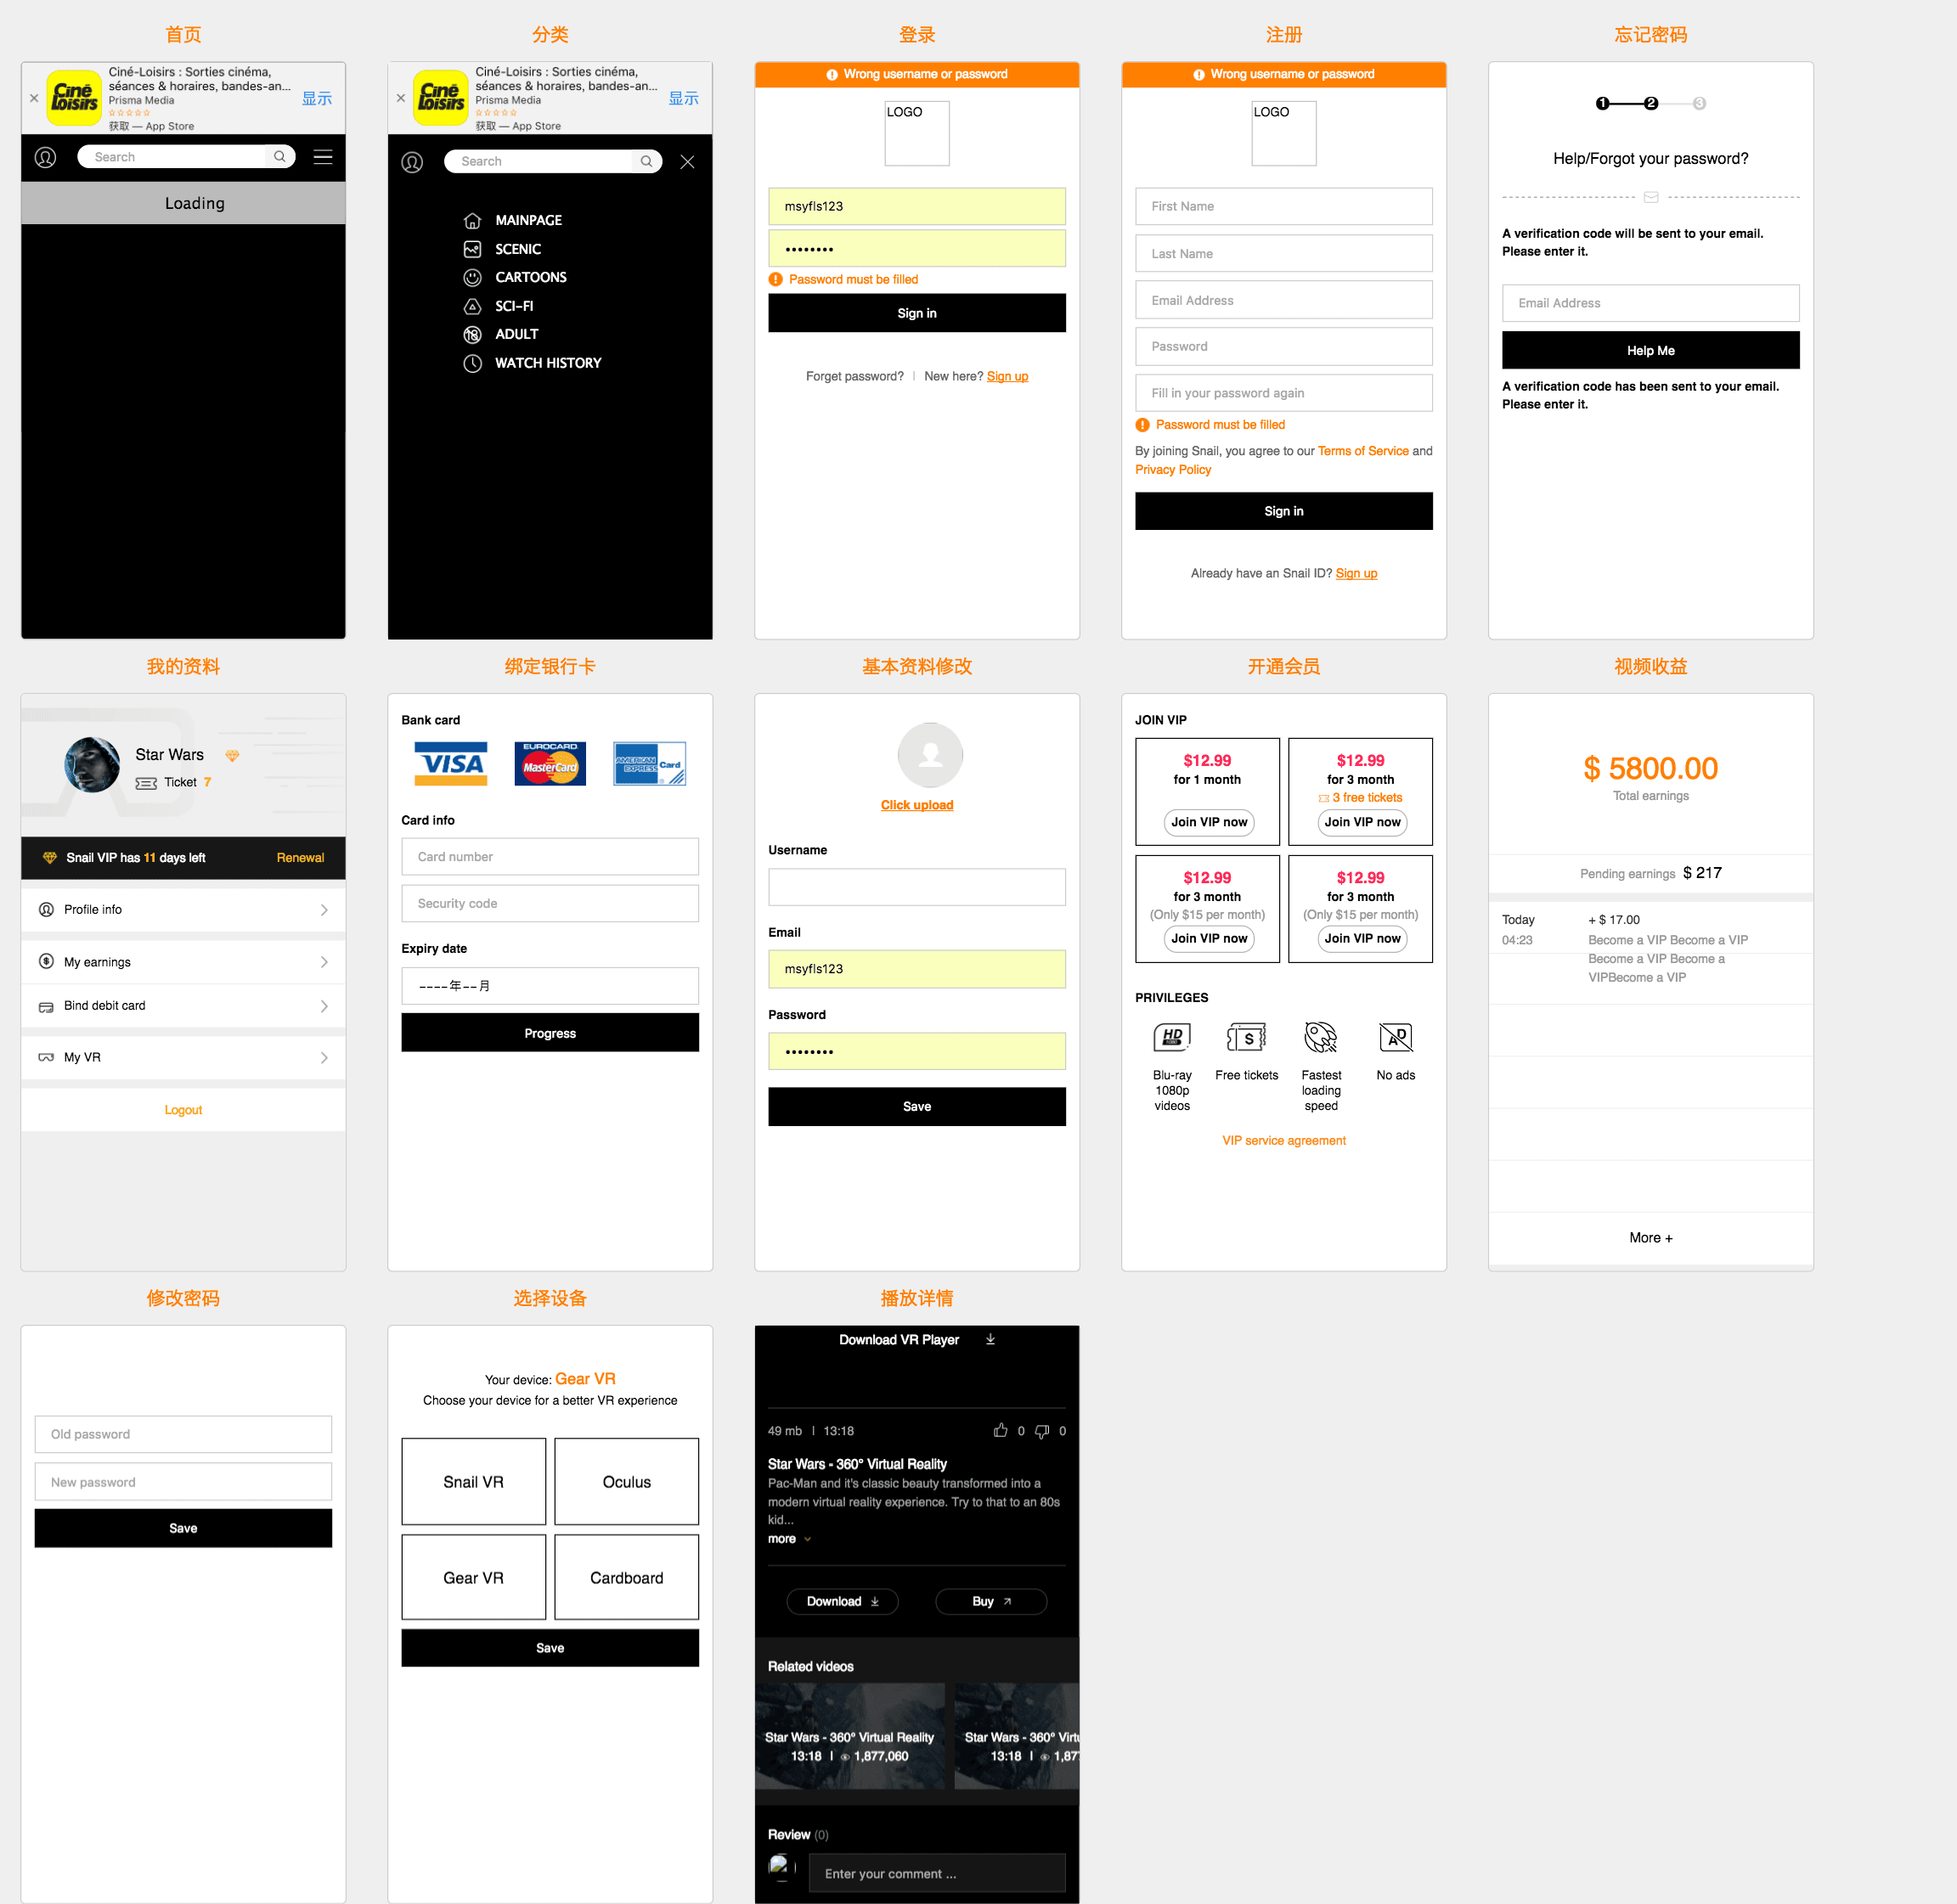
\includegraphics[width=.9\textwidth]{woniu}
}
\caption{移动端全景漫游系统原型}
\label{fig:woniu}
\end{figure}

需求列表如下:
\begin{enumerate}
	\item 满足基本全景漫游功能。因网页环境受限,以直接在浏览器内打开所支持的操作为限,暂不考虑开发多种操作形式功能。
	\item 带有商城功能,实现互动场景的付费/免费使用。
	\item 支持全景视频的播放,基本功能类似普通播放器。
	\item 带有基本的用户设置功能。
\end{enumerate}

根据以上原始需求,从价值需求、功能需求、数据需求等三个角度出发进行需求分析。

\subsection{价值需求分析}
该全景漫游系统的主要用户群为使用计算机或手持移动设备进行网页浏览的青少年群体。其用户特征为对新事物充满好奇心,愿意为良好的用户体验付出金钱成本,但缺点是对事物的专注度低,易于分心。

以该群体作为主要用户对象进行价值评估,按功能和用户的对应需求结合匹配,其价值需求如表\ref{tab:value}。

\begin{table}[htbp]
\centering
\caption{目标群体价值分析}
\vskip 5pt
\begin{tabular}{llll}
\toprule
功能点 & 用户需求 & 价值 \\
\midrule
新鲜感 & 体验到与其他应用不同的内容 & 高 \\
操作性 & 可以方便地了解并获取到所需体验的内容 & 中 \\
可信度 & 能够理解场景传达的信息并作出肯定答复 & 中 \\
丰富性 & 内容类别丰富、有不同难易层次可供选择 & 中 \\
可搜索 & 可以通过文本信息检索需要的项目 & 低 \\
可回溯 & 查看历史回放、收藏夹功能 & 低 \\
社交性 & 体验后愿意与别人分享使用体验 & 高 \\
\bottomrule
\end{tabular}
\label{tab:value}
\end{table}

根据分析,目标群体所期望的是一种不带有过多使用负担、随到随用、用完可离开也可进行分享的交互体验\endnote{陈圆. 手机应用软件界面体验设计研究[D].哈尔滨工程大学,2013.}
。

\subsection{功能需求分析}
据上述价值需求分析可得该全景漫游系统的功能需求,系统内的各种分类或是查找功能等,目的都是通过数据整理来让用户更好地发现场景并与其进行交互,如图\ref{fig:interaction}。经过整理分析以及结合软件开发难度等因素,可得功能需求表\ref{tab:func}。

\begin{figure}[htp]
\centering
\fbox{
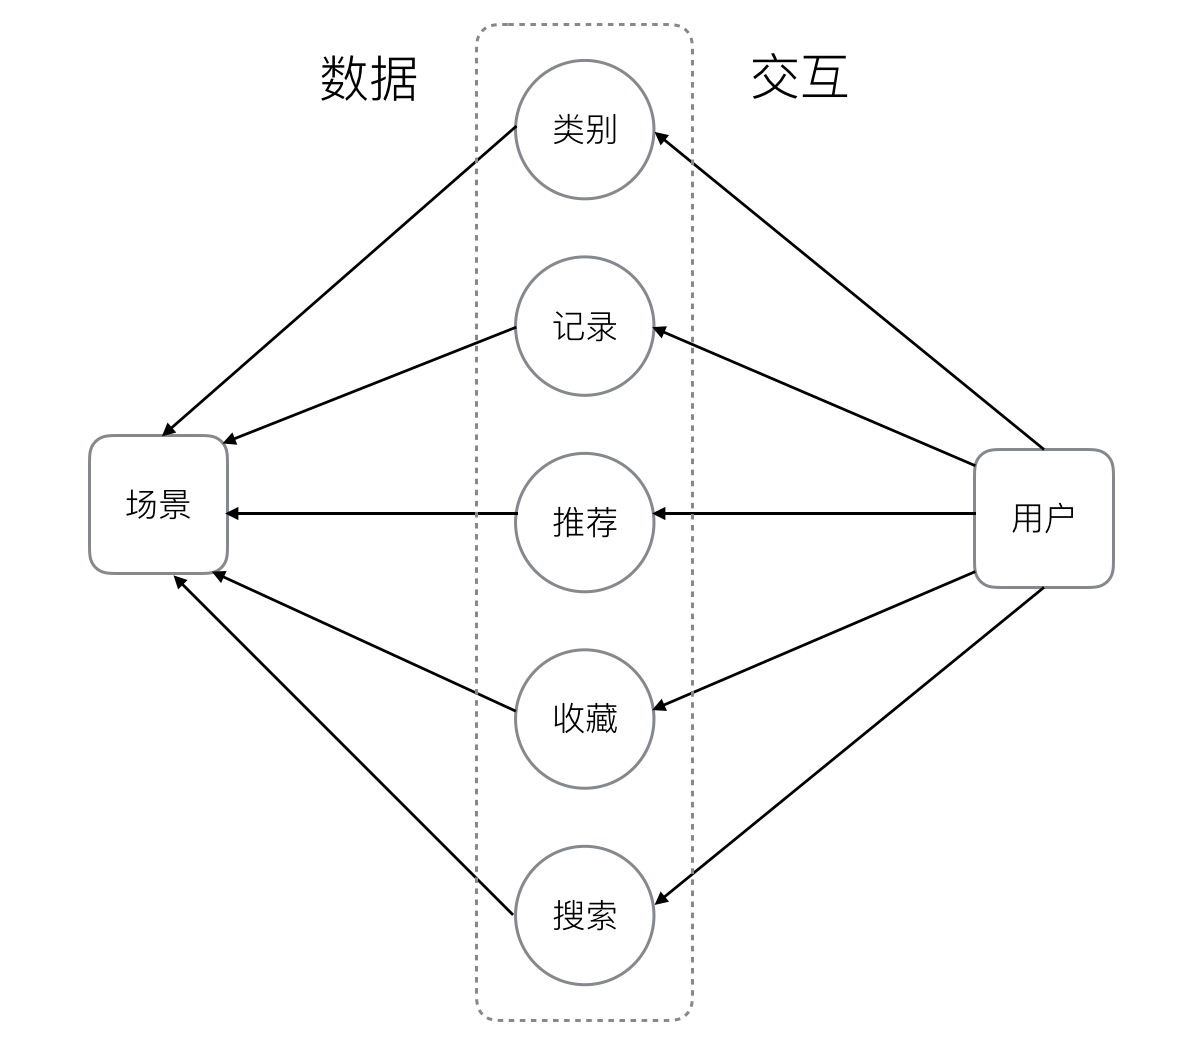
\includegraphics[width=.5\textwidth]{interaction}
}
\caption{用户通过多种形式发现场景}
\label{fig:interaction}
\end{figure}


\begin{table}[htp]
\centering
\caption{功能需求表}
\vskip 5pt
\begin{tabular}{lll}
\toprule
类别 & 功能点 & 描述 \\
\midrule
\multirow{3}{*}{主界面} & 推荐 & 进入推荐场景 \\
& 类别 & 按类别查看场景视频,可翻页,可进入类别界面 \\
& 应用 & 被固定的第三方开发的全景应用 \\
\midrule
\multirow{2}{*}{类别界面} & 列表 & 查看场景视频 \\
& 标签 & 切换类别 \\
\midrule
\multirow{2}{*}{应用界面} & 列表 & 展示第三方应用 \\
& 标签 & 切换类别 \\
\midrule
\multirow{2}{*}{设置界面} & 通用设置 & 提醒、关于 \\
& 个人偏好 & 账户设置、收藏夹、使用记录 \\
\midrule
\multirow{3}{*}{全局导航} & 返回 & 返回上一层 \\
& 主页 & 返回主界面 \\
& 搜索 & 唤起全局或当前类别搜索 \\
\midrule
\multirow{4}{*}{场景} & 定位 & 回到初始角度 \\
& 标签 & 标记为喜爱或讨厌、帮助改进推荐质量 \\
& 分享 & 分享页面至社交媒体 \\
& 解锁 & 解锁付费内容 \\
\bottomrule
\end{tabular}
\label{tab:func}
\end{table}

\subsection{数据需求分析}
根据上述功能需求可知,整个系统中最小的个体单位是场景,数据集合的建立是以场景为中心的。则该全景漫游系统的数据需求以单个场景的数据集出发,进行数据字段的定义,见表\ref{tab:data}。

\begin{table}[htp]
\centering
\caption{场景数据集}
\vskip 5pt
\begin{tabular}{lll}
\toprule
类别 & 字段 & 描述 \\
\midrule
\multirow{4}{*}{基础信息}& 名称 & 场景名称 \\
& 性质 & 视频、游戏、应用等 \\
& 标签 & 场景分类(如科幻、太空等) \\
& 介绍 & 场景简短介绍 \\
\midrule
\multirow{4}{*}{自然信息}& 容量 & 场景占用空间大小,以 kb 计 \\
& 创建日期 & 场景创建日期 \\
& 时长 & 仅对视频场景有效 \\
& 地理信息 & 场景录入地点 \\
\midrule
\multirow{3}{*}{人为信息}& 价格 & 免费、收费、部分收费 \\
& 分级 & 年龄限制、内容限制 \\
& 可用 & 可用或不可用 \\
\bottomrule
\end{tabular}
\label{tab:data}
\end{table}

而作为交互界面,场景是用来服务于使用其的用户的,故数据需求也包含用户信息数据的模型,见表\ref{tab:user}。

\begin{table}[htp]
\centering
\caption{用户数据集}
\vskip 5pt
\begin{tabular}{lll}
\toprule
类别 & 字段 & 描述 \\
\midrule
\multirow{3}{*}{基本信息} & 名称 & 账户名称 \\
& 密码 & 账户密码 \\
& 邮箱 & 账户邮箱 \\
\midrule
\multirow{3}{*}{被动收集信息} & 观看记录 & 场景、时间、时长 \\
& 付费记录 & 场景、应用、视频即其价格 \\
& 操作记录 & 使用场景的有效信息 \\
\midrule
\multirow{3}{*}{主动输入信息} & 标签 & 标记喜恶、收藏 \\
& 偏好设置 & 使用设备、情景模式等 \\
\bottomrule
\end{tabular}
\label{tab:user}
\end{table}

\section{功能架构}
据上述需求分析,该全景漫游系统等功能架构表现两种核心功能:“发现功能”和“场景漫游”。

\subsection{发现功能}
\begin{description}
	\item [浏览功能] 用户在包括主界面内的各种类别界面内浏览场景相关信息,发现自己所想要体验的场景。
	\item [搜索功能] 用户需要即时搜索得到自己想要的信息。
	\item [记录功能] 用户可以查看自己的浏览历史和收藏内容。
	\item [付费功能] 用户需要支付一定成本来查看某些场景或场景的局部。
	\item [自定义功能] 用户可以通过设置来自定义系统偏好。
\end{description}

\subsection{场景漫游功能}

\begin{description}
	\item [漫游功能] 用户可以通过转向、仰头低头、注视等方式漫游整个场景。
	\item [互动功能] 用户可以通过转向、仰头低头、注视等方式漫与场景内特定物件进行互动。
	\item [视频功能] 用户可以以全景的形式观看特殊全景视频。
	\item [标记功能] 用户将场景标记自己的评价、收藏或是分享给其他人。
\end{description}

\section{交互模型}
交互模型即是一系列交互方式、模式、行为的总称,它定义了交互过程中交互的主体对象和行为方式。交互模型并没有准确的定义,因为根据不同的产品而言,交互行为的目的并不相同。例如,对于网站管理员而言,编写并输入网站内容是使用网站的目的,而对于一般浏览者而言,浏览网页上提供的信息则是其在该网站上行为的目的,故从不同角色和视角看待交互模型都会是不同的。而构建交互模型的主要目的则是指导交互设计的进行,则构建一个能同时被用户接受并符合一般软件开发规律的交互模型是十分重要的。

交互模型需要符合用户心智模型并在后续可以方便进行扩充。全景漫游的场景交互模型在前一章节末尾处已经给出,此处不再赘述。在该全景漫游系统中,其系统交互模型如图\ref{fig:scene}。

\begin{figure}[htp]
\centering
\fbox{
  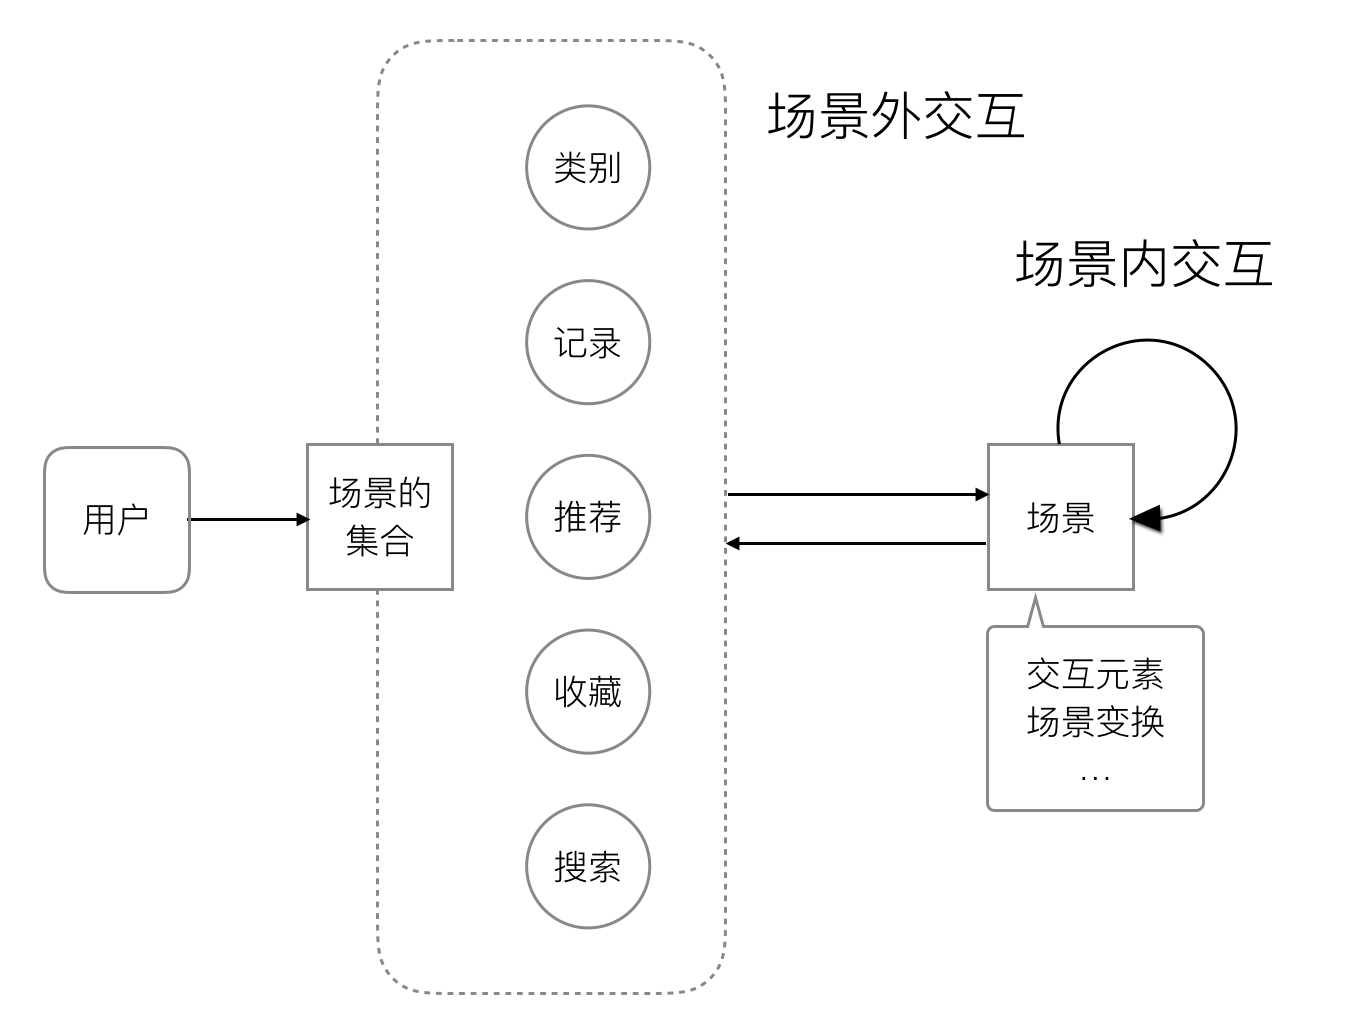
\includegraphics[width=.5\textwidth]{scene}
}
\caption{全景漫游系统的系统交互模型}
\label{fig:scene}
\end{figure}

\section{原型设计}
基于本文提出的全景漫游可视化交互模型,结合上述需求分析与功能架构,我们设计了一个基于网页技术、以开源框架 A-Frame 作为载体的网页版全景漫游系统作为设计原型进行设计制作并验证理论的有效性。

本文将着重从全景漫游系统的导航界面、场景界面、一般功能界面和操作方式等四个方面阐述该设计。
\subsection{类别界面设计}
上方为类别菜单,下边横长条为标签栏,可切换分类。底部为通用导航栏。如图\ref{fig:menu}。

\begin{figure}[htp]
\centering
\fbox{
  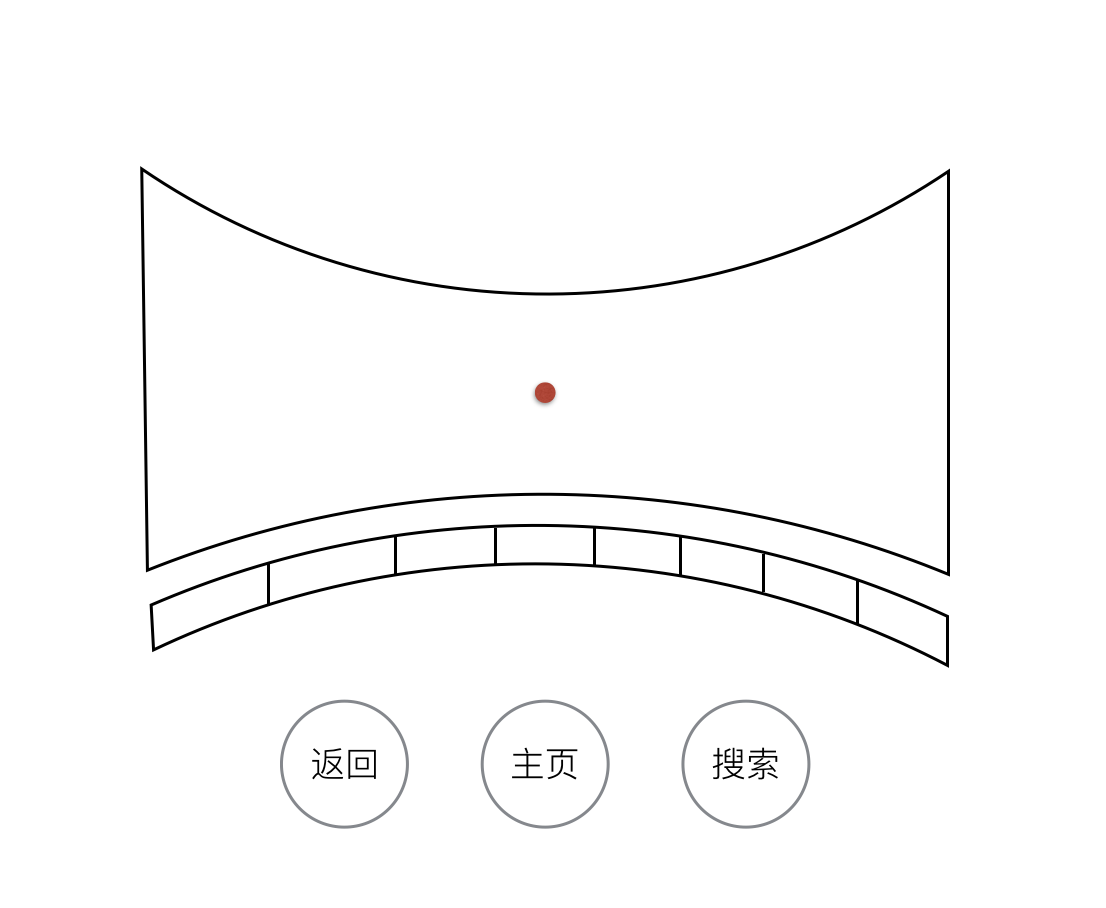
\includegraphics[width=.5\textwidth]{menu}
}
\caption{类别界面设计}
\label{fig:menu}
\end{figure}

\subsection{漫游界面设计}
\begin{itemize}
	\item 漫游界面带有紧急退出区域,只需注视 1~2 秒以上就可以紧急退出场景,避免眩晕加重。
	\item 可通过地面上的指示图标切换场景。
	\item 可通过场景中的热点区域查看详细信息。
\end{itemize}
如图\ref{fig:scenery}。

\begin{figure}[htp]
\centering
\fbox{
  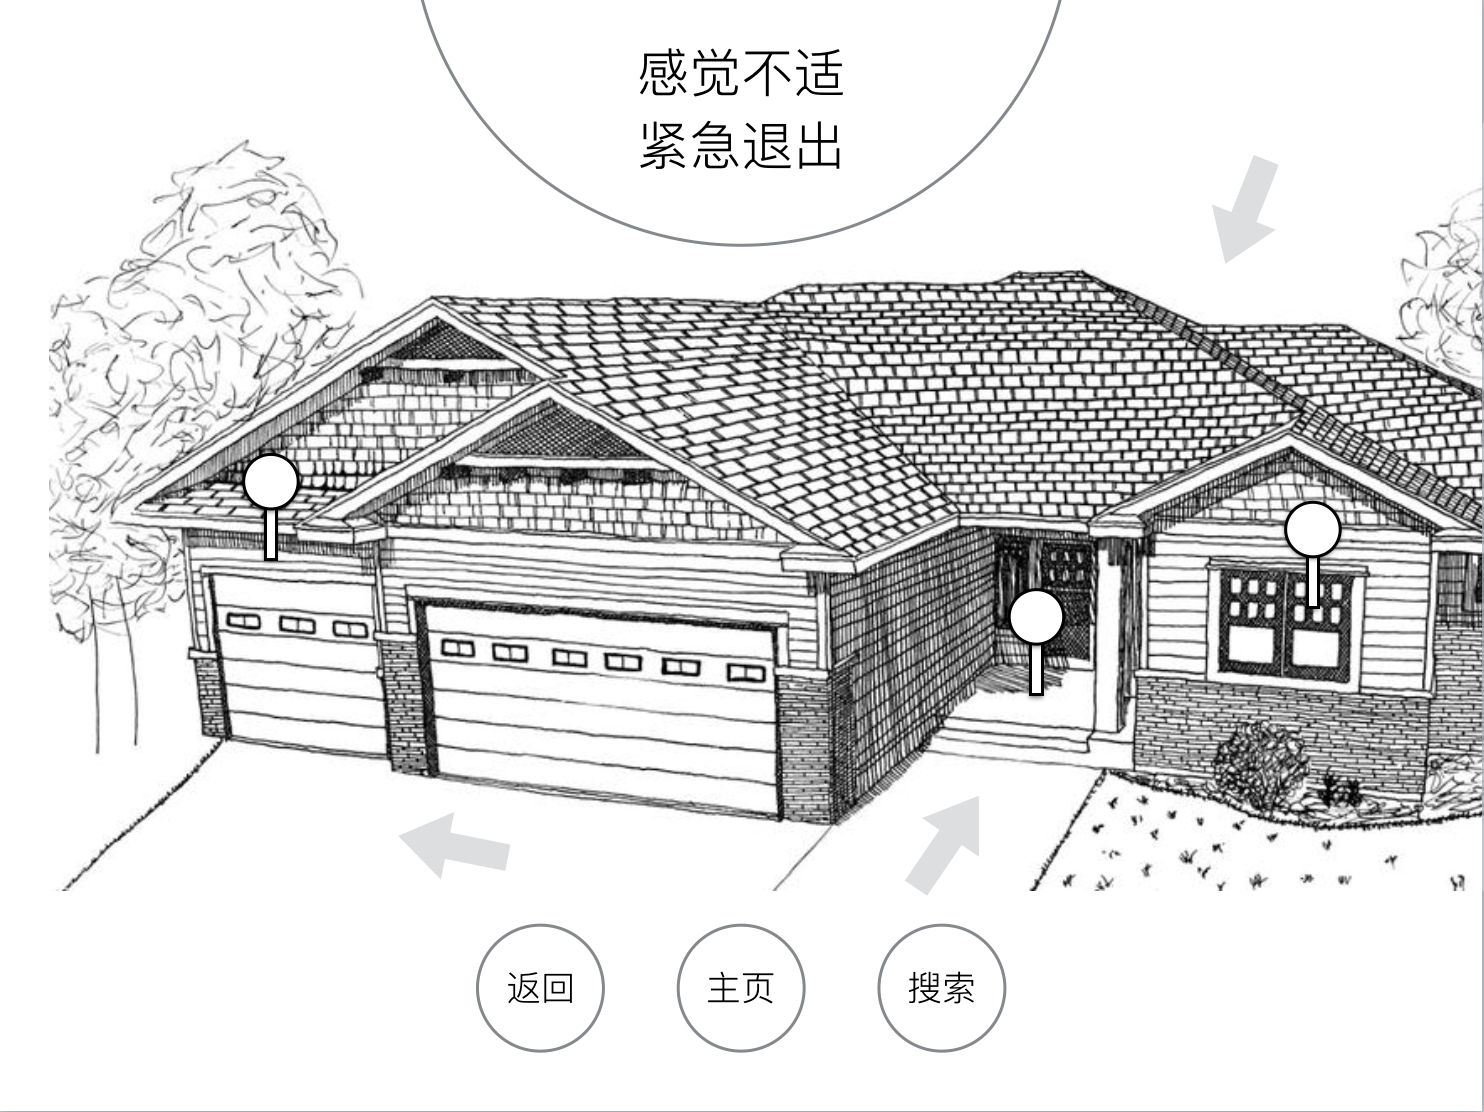
\includegraphics[width=.5\textwidth]{scenery}
}
\caption{漫游界面设计}
\label{fig:scenery}
\end{figure}

\subsection{设置界面设计}
设置界面可通过注视相关范围控件以调节参数,如图\ref{fig:setting}。

\begin{figure}[htp]
\centering
\fbox{
  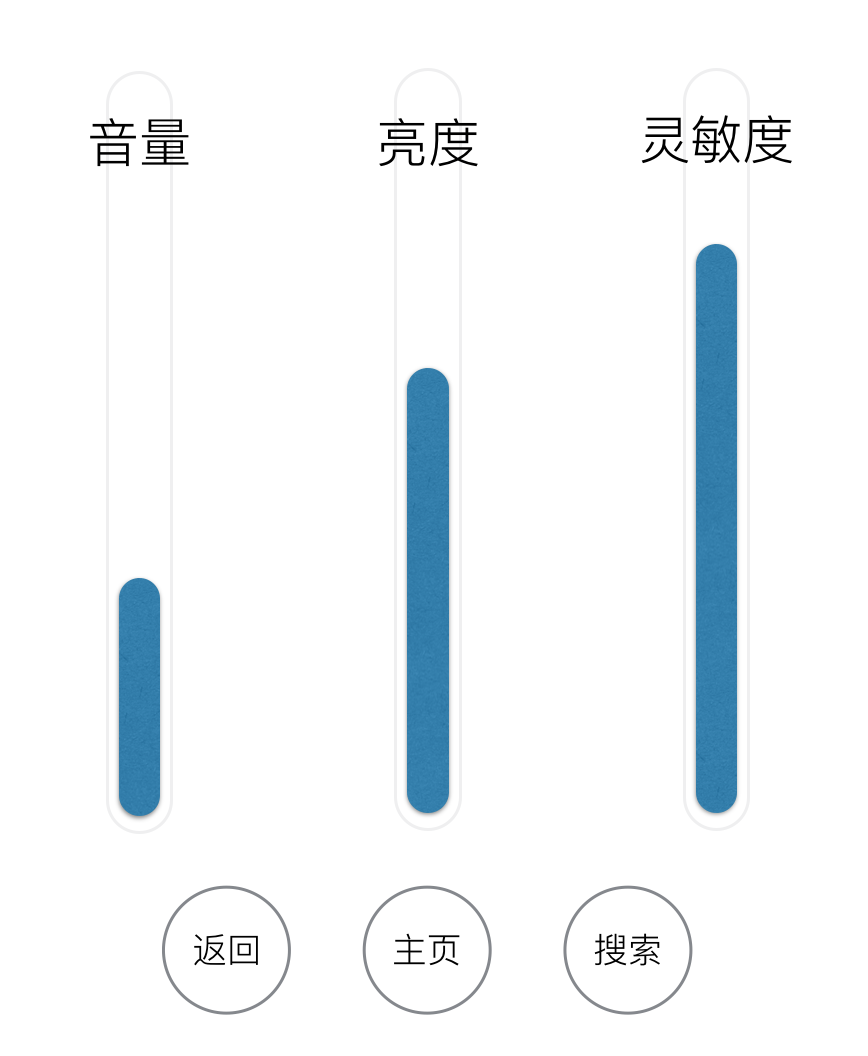
\includegraphics[width=.5\textwidth]{setting}
}
\caption{设置界面设计}
\label{fig:setting}
\end{figure}

\subsection{未完待续}

\section{程序示例}
本全景漫游系统采用 Mozilla 开源的 A-Frame 框架进行开发,可满足普通计算机及移动设备通过浏览器进行使用。

A-Frame 是一款由 Mozilla 开源的网页上用于创建实时虚拟现实体验的框架,其特点是封装性好,功能文档齐全且接受广大开发爱好者共同共享代码\endnote{Srushtika Neelakantam, Tanay Pant. Introduction to A-Frame[J]. 2017.}。其基本实现原理基于现代 HTML5 语言中的画布(Canvas)对象,通过调用底层系统实现高效率的 WebGL 绘图。画布对象的刷新率和延展性均符合全景漫游所必需的基本开发条件,且开发语言与一般网页开发技术类似,对开发团队较为友好,故选用其作为原型展示的应用平台。

开发后生成的原型文件可以通过普通网页进行访问,更可通过 Google Cardboard 配合手机实现简易的全景漫游,其开发便利且容易实现验证。借助以上技术及全景漫游可视化交互理论成果,用户可以真实感受到全景漫游技术带来的体验升级,能够以直观的交互形式与虚拟场景内的事务进行互动,切身体会科技带来的益处\endnote{张小超,王精业. 虚拟场景漫游系统的体系结构分析[J]. 系统仿真学报,2005,(04):917-919.}。
\subsection{示例代码}
实现一个简单的可用鼠标或注视(Fuse)操作的小场景。


\emph{HTML}
\begin{lstlisting}[language=HTML]
<a-scene>
  <a-entity
    id="box" cursor="fuse:true;fuseTimeout:1000"
    geometry="primitive: box"
    material="color: blue">
    <a-box
      src="img/logo.jpg"
      position="0 3 -5"
      rotation="45 0 45"
      scale="2 2 2"
      id="box1">
      <a-animation
        attribute="position"
        begin="focus"
        to="0 2.2 -5"
        direction="normal"
        dur="2000">
      </a-animation>
    </a-box>
  </a-entity>

  <a-camera>
    <a-cursor></a-cursor>
  </a-camera>

  <a-plane 
    position="0 0 -4" 
    rotation="-90 0 0" 
    width="4" 
    height="4" 
    color="#7BC8A4">
  </a-plane>
  <a-sky color="#ECECEC"></a-sky>
</a-scene>
\end{lstlisting} 

\emph{JavaScript}
\begin{lstlisting}{language=JavaScript}
document.querySelector('#box').addEventListener('click', function(e){
  document.querySelector('#box1').emit('focus')
})
\end{lstlisting}

\chapter{待写部分}

\begin{enumerate}
\item{以人为中心,角度,远近等}
\item{上下摆动头部超过一定角度浮现 Docker 栏,例如购物车等}
\end{enumerate}
\theendnotes
\addcontentsline{toc}{chapter}{参考文献}

\end{document}